\documentclass[11pt]{article}
\usepackage{sectsty}
\allsectionsfont{\color{blue}\fontfamily{lmss}\selectfont}
\usepackage{fontspec}
\setmainfont{XCharter}

\usepackage{listings}
\lstset{
basicstyle=\small\ttfamily,
tabsize=8,
columns=flexible,
breaklines=true,
frame=tb,
rulecolor=\color[rgb]{0.8,0.8,0.7},
backgroundcolor=\color[rgb]{1,1,0.91},
postbreak=\raisebox{0ex}[0ex][0ex]{\ensuremath{\color{red}\hookrightarrow\space}}
}
\usepackage{fontawesome}


\usepackage{mdframed}
\newmdenv[
  backgroundcolor=gray,
  fontcolor=white,
  nobreak=true,
]{terminalinput}



\usepackage{parskip}


    \usepackage[breakable]{tcolorbox}
    \usepackage{parskip} % Stop auto-indenting (to mimic markdown behaviour)


    % Basic figure setup, for now with no caption control since it's done
    % automatically by Pandoc (which extracts ![](path) syntax from Markdown).
    \usepackage{graphicx}
    % Maintain compatibility with old templates. Remove in nbconvert 6.0
    \let\Oldincludegraphics\includegraphics
    % Ensure that by default, figures have no caption (until we provide a
    % proper Figure object with a Caption API and a way to capture that
    % in the conversion process - todo).
    \usepackage{caption}
    \DeclareCaptionFormat{nocaption}{}
    \captionsetup{format=nocaption,aboveskip=0pt,belowskip=0pt}

    \usepackage{float}
    \floatplacement{figure}{H} % forces figures to be placed at the correct location
    \usepackage{xcolor} % Allow colors to be defined
    \usepackage{enumerate} % Needed for markdown enumerations to work
    \usepackage{geometry} % Used to adjust the document margins
    \usepackage{amsmath} % Equations
    \usepackage{amssymb} % Equations
    \usepackage{textcomp} % defines textquotesingle
    % Hack from http://tex.stackexchange.com/a/47451/13684:
    \AtBeginDocument{%
        \def\PYZsq{\textquotesingle}% Upright quotes in Pygmentized code
    }
    \usepackage{upquote} % Upright quotes for verbatim code
    \usepackage{eurosym} % defines \euro

    \usepackage{iftex}
    \ifPDFTeX
        \usepackage[T1]{fontenc}
        \IfFileExists{alphabeta.sty}{
              \usepackage{alphabeta}
          }{
              \usepackage[mathletters]{ucs}
              \usepackage[utf8x]{inputenc}
          }
    \else
        \usepackage{fontspec}
        \usepackage{unicode-math}
    \fi

    \usepackage{fancyvrb} % verbatim replacement that allows latex
    \usepackage{grffile} % extends the file name processing of package graphics
                         % to support a larger range
    \makeatletter % fix for old versions of grffile with XeLaTeX
    \@ifpackagelater{grffile}{2019/11/01}
    {
      % Do nothing on new versions
    }
    {
      \def\Gread@@xetex#1{%
        \IfFileExists{"\Gin@base".bb}%
        {\Gread@eps{\Gin@base.bb}}%
        {\Gread@@xetex@aux#1}%
      }
    }
    \makeatother
    \usepackage[Export]{adjustbox} % Used to constrain images to a maximum size
    \adjustboxset{max size={0.9\linewidth}{0.9\paperheight}}

    % The hyperref package gives us a pdf with properly built
    % internal navigation ('pdf bookmarks' for the table of contents,
    % internal cross-reference links, web links for URLs, etc.)
    \usepackage{hyperref}
    % The default LaTeX title has an obnoxious amount of whitespace. By default,
    % titling removes some of it. It also provides customization options.
    \usepackage{titling}
    \usepackage{longtable} % longtable support required by pandoc >1.10
    \usepackage{booktabs}  % table support for pandoc > 1.12.2
    \usepackage{array}     % table support for pandoc >= 2.11.3
    \usepackage{calc}      % table minipage width calculation for pandoc >= 2.11.1
    \usepackage[inline]{enumitem} % IRkernel/repr support (it uses the enumerate* environment)
    \usepackage[normalem]{ulem} % ulem is needed to support strikethroughs (\sout)
                                % normalem makes italics be italics, not underlines
    \usepackage{mathrsfs}



    % Colors for the hyperref package
    \definecolor{urlcolor}{rgb}{0,.145,.698}
    \definecolor{linkcolor}{rgb}{.71,0.21,0.01}
    \definecolor{citecolor}{rgb}{.12,.54,.11}

    % ANSI colors
    \definecolor{ansi-black}{HTML}{3E424D}
    \definecolor{ansi-black-intense}{HTML}{282C36}
    \definecolor{ansi-red}{HTML}{E75C58}
    \definecolor{ansi-red-intense}{HTML}{B22B31}
    \definecolor{ansi-green}{HTML}{00A250}
    \definecolor{ansi-green-intense}{HTML}{007427}
    \definecolor{ansi-yellow}{HTML}{DDB62B}
    \definecolor{ansi-yellow-intense}{HTML}{B27D12}
    \definecolor{ansi-blue}{HTML}{208FFB}
    \definecolor{ansi-blue-intense}{HTML}{0065CA}
    \definecolor{ansi-magenta}{HTML}{D160C4}
    \definecolor{ansi-magenta-intense}{HTML}{A03196}
    \definecolor{ansi-cyan}{HTML}{60C6C8}
    \definecolor{ansi-cyan-intense}{HTML}{258F8F}
    \definecolor{ansi-white}{HTML}{C5C1B4}
    \definecolor{ansi-white-intense}{HTML}{A1A6B2}
    \definecolor{ansi-default-inverse-fg}{HTML}{FFFFFF}
    \definecolor{ansi-default-inverse-bg}{HTML}{000000}

    % common color for the border for error outputs.
    \definecolor{outerrorbackground}{HTML}{FFDFDF}

    % commands and environments needed by pandoc snippets
    % extracted from the output of `pandoc -s`
    \providecommand{\tightlist}{%
      \setlength{\itemsep}{0pt}\setlength{\parskip}{0pt}}
    \DefineVerbatimEnvironment{Highlighting}{Verbatim}{commandchars=\\\{\}}
    % Add ',fontsize=\small' for more characters per line
    \newenvironment{Shaded}{}{}
    \newcommand{\KeywordTok}[1]{\textcolor[rgb]{0.00,0.44,0.13}{\textbf{{#1}}}}
    \newcommand{\DataTypeTok}[1]{\textcolor[rgb]{0.56,0.13,0.00}{{#1}}}
    \newcommand{\DecValTok}[1]{\textcolor[rgb]{0.25,0.63,0.44}{{#1}}}
    \newcommand{\BaseNTok}[1]{\textcolor[rgb]{0.25,0.63,0.44}{{#1}}}
    \newcommand{\FloatTok}[1]{\textcolor[rgb]{0.25,0.63,0.44}{{#1}}}
    \newcommand{\CharTok}[1]{\textcolor[rgb]{0.25,0.44,0.63}{{#1}}}
    \newcommand{\StringTok}[1]{\textcolor[rgb]{0.25,0.44,0.63}{{#1}}}
    \newcommand{\CommentTok}[1]{\textcolor[rgb]{0.38,0.63,0.69}{\textit{{#1}}}}
    \newcommand{\OtherTok}[1]{\textcolor[rgb]{0.00,0.44,0.13}{{#1}}}
    \newcommand{\AlertTok}[1]{\textcolor[rgb]{1.00,0.00,0.00}{\textbf{{#1}}}}
    \newcommand{\FunctionTok}[1]{\textcolor[rgb]{0.02,0.16,0.49}{{#1}}}
    \newcommand{\RegionMarkerTok}[1]{{#1}}
    \newcommand{\ErrorTok}[1]{\textcolor[rgb]{1.00,0.00,0.00}{\textbf{{#1}}}}
    \newcommand{\NormalTok}[1]{{#1}}

    % Additional commands for more recent versions of Pandoc
    \newcommand{\ConstantTok}[1]{\textcolor[rgb]{0.53,0.00,0.00}{{#1}}}
    \newcommand{\SpecialCharTok}[1]{\textcolor[rgb]{0.25,0.44,0.63}{{#1}}}
    \newcommand{\VerbatimStringTok}[1]{\textcolor[rgb]{0.25,0.44,0.63}{{#1}}}
    \newcommand{\SpecialStringTok}[1]{\textcolor[rgb]{0.73,0.40,0.53}{{#1}}}
    \newcommand{\ImportTok}[1]{{#1}}
    \newcommand{\DocumentationTok}[1]{\textcolor[rgb]{0.73,0.13,0.13}{\textit{{#1}}}}
    \newcommand{\AnnotationTok}[1]{\textcolor[rgb]{0.38,0.63,0.69}{\textbf{\textit{{#1}}}}}
    \newcommand{\CommentVarTok}[1]{\textcolor[rgb]{0.38,0.63,0.69}{\textbf{\textit{{#1}}}}}
    \newcommand{\VariableTok}[1]{\textcolor[rgb]{0.10,0.09,0.49}{{#1}}}
    \newcommand{\ControlFlowTok}[1]{\textcolor[rgb]{0.00,0.44,0.13}{\textbf{{#1}}}}
    \newcommand{\OperatorTok}[1]{\textcolor[rgb]{0.40,0.40,0.40}{{#1}}}
    \newcommand{\BuiltInTok}[1]{{#1}}
    \newcommand{\ExtensionTok}[1]{{#1}}
    \newcommand{\PreprocessorTok}[1]{\textcolor[rgb]{0.74,0.48,0.00}{{#1}}}
    \newcommand{\AttributeTok}[1]{\textcolor[rgb]{0.49,0.56,0.16}{{#1}}}
    \newcommand{\InformationTok}[1]{\textcolor[rgb]{0.38,0.63,0.69}{\textbf{\textit{{#1}}}}}
    \newcommand{\WarningTok}[1]{\textcolor[rgb]{0.38,0.63,0.69}{\textbf{\textit{{#1}}}}}


    % Define a nice break command that doesn't care if a line doesn't already
    % exist.
    \def\br{\hspace*{\fill} \\* }
    % Math Jax compatibility definitions
    \def\gt{>}
    \def\lt{<}
    \let\Oldtex\TeX
    \let\Oldlatex\LaTeX
    \renewcommand{\TeX}{\textrm{\Oldtex}}
    \renewcommand{\LaTeX}{\textrm{\Oldlatex}}
    % Document parameters
    % Document title
    \title{index}





% Pygments definitions
\makeatletter
\def\PY@reset{\let\PY@it=\relax \let\PY@bf=\relax%
    \let\PY@ul=\relax \let\PY@tc=\relax%
    \let\PY@bc=\relax \let\PY@ff=\relax}
\def\PY@tok#1{\csname PY@tok@#1\endcsname}
\def\PY@toks#1+{\ifx\relax#1\empty\else%
    \PY@tok{#1}\expandafter\PY@toks\fi}
\def\PY@do#1{\PY@bc{\PY@tc{\PY@ul{%
    \PY@it{\PY@bf{\PY@ff{#1}}}}}}}
\def\PY#1#2{\PY@reset\PY@toks#1+\relax+\PY@do{#2}}

\@namedef{PY@tok@w}{\def\PY@tc##1{\textcolor[rgb]{0.73,0.73,0.73}{##1}}}
\@namedef{PY@tok@c}{\let\PY@it=\textit\def\PY@tc##1{\textcolor[rgb]{0.24,0.48,0.48}{##1}}}
\@namedef{PY@tok@cp}{\def\PY@tc##1{\textcolor[rgb]{0.61,0.40,0.00}{##1}}}
\@namedef{PY@tok@k}{\let\PY@bf=\textbf\def\PY@tc##1{\textcolor[rgb]{0.00,0.50,0.00}{##1}}}
\@namedef{PY@tok@kp}{\def\PY@tc##1{\textcolor[rgb]{0.00,0.50,0.00}{##1}}}
\@namedef{PY@tok@kt}{\def\PY@tc##1{\textcolor[rgb]{0.69,0.00,0.25}{##1}}}
\@namedef{PY@tok@o}{\def\PY@tc##1{\textcolor[rgb]{0.40,0.40,0.40}{##1}}}
\@namedef{PY@tok@ow}{\let\PY@bf=\textbf\def\PY@tc##1{\textcolor[rgb]{0.67,0.13,1.00}{##1}}}
\@namedef{PY@tok@nb}{\def\PY@tc##1{\textcolor[rgb]{0.00,0.50,0.00}{##1}}}
\@namedef{PY@tok@nf}{\def\PY@tc##1{\textcolor[rgb]{0.00,0.00,1.00}{##1}}}
\@namedef{PY@tok@nc}{\let\PY@bf=\textbf\def\PY@tc##1{\textcolor[rgb]{0.00,0.00,1.00}{##1}}}
\@namedef{PY@tok@nn}{\let\PY@bf=\textbf\def\PY@tc##1{\textcolor[rgb]{0.00,0.00,1.00}{##1}}}
\@namedef{PY@tok@ne}{\let\PY@bf=\textbf\def\PY@tc##1{\textcolor[rgb]{0.80,0.25,0.22}{##1}}}
\@namedef{PY@tok@nv}{\def\PY@tc##1{\textcolor[rgb]{0.10,0.09,0.49}{##1}}}
\@namedef{PY@tok@no}{\def\PY@tc##1{\textcolor[rgb]{0.53,0.00,0.00}{##1}}}
\@namedef{PY@tok@nl}{\def\PY@tc##1{\textcolor[rgb]{0.46,0.46,0.00}{##1}}}
\@namedef{PY@tok@ni}{\let\PY@bf=\textbf\def\PY@tc##1{\textcolor[rgb]{0.44,0.44,0.44}{##1}}}
\@namedef{PY@tok@na}{\def\PY@tc##1{\textcolor[rgb]{0.41,0.47,0.13}{##1}}}
\@namedef{PY@tok@nt}{\let\PY@bf=\textbf\def\PY@tc##1{\textcolor[rgb]{0.00,0.50,0.00}{##1}}}
\@namedef{PY@tok@nd}{\def\PY@tc##1{\textcolor[rgb]{0.67,0.13,1.00}{##1}}}
\@namedef{PY@tok@s}{\def\PY@tc##1{\textcolor[rgb]{0.73,0.13,0.13}{##1}}}
\@namedef{PY@tok@sd}{\let\PY@it=\textit\def\PY@tc##1{\textcolor[rgb]{0.73,0.13,0.13}{##1}}}
\@namedef{PY@tok@si}{\let\PY@bf=\textbf\def\PY@tc##1{\textcolor[rgb]{0.64,0.35,0.47}{##1}}}
\@namedef{PY@tok@se}{\let\PY@bf=\textbf\def\PY@tc##1{\textcolor[rgb]{0.67,0.36,0.12}{##1}}}
\@namedef{PY@tok@sr}{\def\PY@tc##1{\textcolor[rgb]{0.64,0.35,0.47}{##1}}}
\@namedef{PY@tok@ss}{\def\PY@tc##1{\textcolor[rgb]{0.10,0.09,0.49}{##1}}}
\@namedef{PY@tok@sx}{\def\PY@tc##1{\textcolor[rgb]{0.00,0.50,0.00}{##1}}}
\@namedef{PY@tok@m}{\def\PY@tc##1{\textcolor[rgb]{0.40,0.40,0.40}{##1}}}
\@namedef{PY@tok@gh}{\let\PY@bf=\textbf\def\PY@tc##1{\textcolor[rgb]{0.00,0.00,0.50}{##1}}}
\@namedef{PY@tok@gu}{\let\PY@bf=\textbf\def\PY@tc##1{\textcolor[rgb]{0.50,0.00,0.50}{##1}}}
\@namedef{PY@tok@gd}{\def\PY@tc##1{\textcolor[rgb]{0.63,0.00,0.00}{##1}}}
\@namedef{PY@tok@gi}{\def\PY@tc##1{\textcolor[rgb]{0.00,0.52,0.00}{##1}}}
\@namedef{PY@tok@gr}{\def\PY@tc##1{\textcolor[rgb]{0.89,0.00,0.00}{##1}}}
\@namedef{PY@tok@ge}{\let\PY@it=\textit}
\@namedef{PY@tok@gs}{\let\PY@bf=\textbf}
\@namedef{PY@tok@gp}{\let\PY@bf=\textbf\def\PY@tc##1{\textcolor[rgb]{0.00,0.00,0.50}{##1}}}
\@namedef{PY@tok@go}{\def\PY@tc##1{\textcolor[rgb]{0.44,0.44,0.44}{##1}}}
\@namedef{PY@tok@gt}{\def\PY@tc##1{\textcolor[rgb]{0.00,0.27,0.87}{##1}}}
\@namedef{PY@tok@err}{\def\PY@bc##1{{\setlength{\fboxsep}{\string -\fboxrule}\fcolorbox[rgb]{1.00,0.00,0.00}{1,1,1}{\strut ##1}}}}
\@namedef{PY@tok@kc}{\let\PY@bf=\textbf\def\PY@tc##1{\textcolor[rgb]{0.00,0.50,0.00}{##1}}}
\@namedef{PY@tok@kd}{\let\PY@bf=\textbf\def\PY@tc##1{\textcolor[rgb]{0.00,0.50,0.00}{##1}}}
\@namedef{PY@tok@kn}{\let\PY@bf=\textbf\def\PY@tc##1{\textcolor[rgb]{0.00,0.50,0.00}{##1}}}
\@namedef{PY@tok@kr}{\let\PY@bf=\textbf\def\PY@tc##1{\textcolor[rgb]{0.00,0.50,0.00}{##1}}}
\@namedef{PY@tok@bp}{\def\PY@tc##1{\textcolor[rgb]{0.00,0.50,0.00}{##1}}}
\@namedef{PY@tok@fm}{\def\PY@tc##1{\textcolor[rgb]{0.00,0.00,1.00}{##1}}}
\@namedef{PY@tok@vc}{\def\PY@tc##1{\textcolor[rgb]{0.10,0.09,0.49}{##1}}}
\@namedef{PY@tok@vg}{\def\PY@tc##1{\textcolor[rgb]{0.10,0.09,0.49}{##1}}}
\@namedef{PY@tok@vi}{\def\PY@tc##1{\textcolor[rgb]{0.10,0.09,0.49}{##1}}}
\@namedef{PY@tok@vm}{\def\PY@tc##1{\textcolor[rgb]{0.10,0.09,0.49}{##1}}}
\@namedef{PY@tok@sa}{\def\PY@tc##1{\textcolor[rgb]{0.73,0.13,0.13}{##1}}}
\@namedef{PY@tok@sb}{\def\PY@tc##1{\textcolor[rgb]{0.73,0.13,0.13}{##1}}}
\@namedef{PY@tok@sc}{\def\PY@tc##1{\textcolor[rgb]{0.73,0.13,0.13}{##1}}}
\@namedef{PY@tok@dl}{\def\PY@tc##1{\textcolor[rgb]{0.73,0.13,0.13}{##1}}}
\@namedef{PY@tok@s2}{\def\PY@tc##1{\textcolor[rgb]{0.73,0.13,0.13}{##1}}}
\@namedef{PY@tok@sh}{\def\PY@tc##1{\textcolor[rgb]{0.73,0.13,0.13}{##1}}}
\@namedef{PY@tok@s1}{\def\PY@tc##1{\textcolor[rgb]{0.73,0.13,0.13}{##1}}}
\@namedef{PY@tok@mb}{\def\PY@tc##1{\textcolor[rgb]{0.40,0.40,0.40}{##1}}}
\@namedef{PY@tok@mf}{\def\PY@tc##1{\textcolor[rgb]{0.40,0.40,0.40}{##1}}}
\@namedef{PY@tok@mh}{\def\PY@tc##1{\textcolor[rgb]{0.40,0.40,0.40}{##1}}}
\@namedef{PY@tok@mi}{\def\PY@tc##1{\textcolor[rgb]{0.40,0.40,0.40}{##1}}}
\@namedef{PY@tok@il}{\def\PY@tc##1{\textcolor[rgb]{0.40,0.40,0.40}{##1}}}
\@namedef{PY@tok@mo}{\def\PY@tc##1{\textcolor[rgb]{0.40,0.40,0.40}{##1}}}
\@namedef{PY@tok@ch}{\let\PY@it=\textit\def\PY@tc##1{\textcolor[rgb]{0.24,0.48,0.48}{##1}}}
\@namedef{PY@tok@cm}{\let\PY@it=\textit\def\PY@tc##1{\textcolor[rgb]{0.24,0.48,0.48}{##1}}}
\@namedef{PY@tok@cpf}{\let\PY@it=\textit\def\PY@tc##1{\textcolor[rgb]{0.24,0.48,0.48}{##1}}}
\@namedef{PY@tok@c1}{\let\PY@it=\textit\def\PY@tc##1{\textcolor[rgb]{0.24,0.48,0.48}{##1}}}
\@namedef{PY@tok@cs}{\let\PY@it=\textit\def\PY@tc##1{\textcolor[rgb]{0.24,0.48,0.48}{##1}}}

\def\PYZbs{\char`\\}
\def\PYZus{\char`\_}
\def\PYZob{\char`\{}
\def\PYZcb{\char`\}}
\def\PYZca{\char`\^}
\def\PYZam{\char`\&}
\def\PYZlt{\char`\<}
\def\PYZgt{\char`\>}
\def\PYZsh{\char`\#}
\def\PYZpc{\char`\%}
\def\PYZdl{\char`\$}
\def\PYZhy{\char`\-}
\def\PYZsq{\char`\'}
\def\PYZdq{\char`\"}
\def\PYZti{\char`\~}
% for compatibility with earlier versions
\def\PYZat{@}
\def\PYZlb{[}
\def\PYZrb{]}
\makeatother


    % For linebreaks inside Verbatim environment from package fancyvrb.
    \makeatletter
        \newbox\Wrappedcontinuationbox
        \newbox\Wrappedvisiblespacebox
        \newcommand*\Wrappedvisiblespace {\textcolor{red}{\textvisiblespace}}
        \newcommand*\Wrappedcontinuationsymbol {\textcolor{red}{\llap{\tiny$\m@th\hookrightarrow$}}}
        \newcommand*\Wrappedcontinuationindent {3ex }
        \newcommand*\Wrappedafterbreak {\kern\Wrappedcontinuationindent\copy\Wrappedcontinuationbox}
        % Take advantage of the already applied Pygments mark-up to insert
        % potential linebreaks for TeX processing.
        %        {, <, #, %, $, ' and ": go to next line.
        %        _, }, ^, &, >, - and ~: stay at end of broken line.
        % Use of \textquotesingle for straight quote.
        \newcommand*\Wrappedbreaksatspecials {%
            \def\PYGZus{\discretionary{\char`\_}{\Wrappedafterbreak}{\char`\_}}%
            \def\PYGZob{\discretionary{}{\Wrappedafterbreak\char`\{}{\char`\{}}%
            \def\PYGZcb{\discretionary{\char`\}}{\Wrappedafterbreak}{\char`\}}}%
            \def\PYGZca{\discretionary{\char`\^}{\Wrappedafterbreak}{\char`\^}}%
            \def\PYGZam{\discretionary{\char`\&}{\Wrappedafterbreak}{\char`\&}}%
            \def\PYGZlt{\discretionary{}{\Wrappedafterbreak\char`\<}{\char`\<}}%
            \def\PYGZgt{\discretionary{\char`\>}{\Wrappedafterbreak}{\char`\>}}%
            \def\PYGZsh{\discretionary{}{\Wrappedafterbreak\char`\#}{\char`\#}}%
            \def\PYGZpc{\discretionary{}{\Wrappedafterbreak\char`\%}{\char`\%}}%
            \def\PYGZdl{\discretionary{}{\Wrappedafterbreak\char`\$}{\char`\$}}%
            \def\PYGZhy{\discretionary{\char`\-}{\Wrappedafterbreak}{\char`\-}}%
            \def\PYGZsq{\discretionary{}{\Wrappedafterbreak\textquotesingle}{\textquotesingle}}%
            \def\PYGZdq{\discretionary{}{\Wrappedafterbreak\char`\"}{\char`\"}}%
            \def\PYGZti{\discretionary{\char`\~}{\Wrappedafterbreak}{\char`\~}}%
        }
        % Some characters . , ; ? ! / are not pygmentized.
        % This macro makes them "active" and they will insert potential linebreaks
        \newcommand*\Wrappedbreaksatpunct {%
            \lccode`\~`\.\lowercase{\def~}{\discretionary{\hbox{\char`\.}}{\Wrappedafterbreak}{\hbox{\char`\.}}}%
            \lccode`\~`\,\lowercase{\def~}{\discretionary{\hbox{\char`\,}}{\Wrappedafterbreak}{\hbox{\char`\,}}}%
            \lccode`\~`\;\lowercase{\def~}{\discretionary{\hbox{\char`\;}}{\Wrappedafterbreak}{\hbox{\char`\;}}}%
            \lccode`\~`\:\lowercase{\def~}{\discretionary{\hbox{\char`\:}}{\Wrappedafterbreak}{\hbox{\char`\:}}}%
            \lccode`\~`\?\lowercase{\def~}{\discretionary{\hbox{\char`\?}}{\Wrappedafterbreak}{\hbox{\char`\?}}}%
            \lccode`\~`\!\lowercase{\def~}{\discretionary{\hbox{\char`\!}}{\Wrappedafterbreak}{\hbox{\char`\!}}}%
            \lccode`\~`\/\lowercase{\def~}{\discretionary{\hbox{\char`\/}}{\Wrappedafterbreak}{\hbox{\char`\/}}}%
            \catcode`\.\active
            \catcode`\,\active
            \catcode`\;\active
            \catcode`\:\active
            \catcode`\?\active
            \catcode`\!\active
            \catcode`\/\active
            \lccode`\~`\~
        }
    \makeatother

    \let\OriginalVerbatim=\Verbatim
    \makeatletter
    \renewcommand{\Verbatim}[1][1]{%
        %\parskip\z@skip
        \sbox\Wrappedcontinuationbox {\Wrappedcontinuationsymbol}%
        \sbox\Wrappedvisiblespacebox {\FV@SetupFont\Wrappedvisiblespace}%
        \def\FancyVerbFormatLine ##1{\hsize\linewidth
            \vtop{\raggedright\hyphenpenalty\z@\exhyphenpenalty\z@
                \doublehyphendemerits\z@\finalhyphendemerits\z@
                \strut ##1\strut}%
        }%
        % If the linebreak is at a space, the latter will be displayed as visible
        % space at end of first line, and a continuation symbol starts next line.
        % Stretch/shrink are however usually zero for typewriter font.
        \def\FV@Space {%
            \nobreak\hskip\z@ plus\fontdimen3\font minus\fontdimen4\font
            \discretionary{\copy\Wrappedvisiblespacebox}{\Wrappedafterbreak}
            {\kern\fontdimen2\font}%
        }%

        % Allow breaks at special characters using \PYG... macros.
        \Wrappedbreaksatspecials
        % Breaks at punctuation characters . , ; ? ! and / need catcode=\active
        \OriginalVerbatim[#1,codes*=\Wrappedbreaksatpunct]%
    }
    \makeatother

    % Exact colors from NB
    \definecolor{incolor}{HTML}{303F9F}
    \definecolor{outcolor}{HTML}{D84315}
    \definecolor{cellborder}{HTML}{CFCFCF}
    \definecolor{cellbackground}{HTML}{F7F7F7}

    % prompt
    \makeatletter
    \newcommand{\boxspacing}{\kern\kvtcb@left@rule\kern\kvtcb@boxsep}
    \makeatother
    \newcommand{\prompt}[4]{
        {\ttfamily\llap{{\color{blue}\LARGE\faKeyboardO\hspace{3pt}#4}}\vspace{-\baselineskip}}
    }



    % Prevent overflowing lines due to hard-to-break entities
    \sloppy
    % Setup hyperref package
    \hypersetup{
      breaklinks=true,  % so long urls are correctly broken across lines
      colorlinks=true,
      urlcolor=urlcolor,
      linkcolor=linkcolor,
      citecolor=citecolor,
      }
    % Slightly bigger margins than the latex defaults

    \geometry{verbose,tmargin=1in,bmargin=1in,lmargin=1in,rmargin=1in}



\renewcommand{\PY}[2]{{#2}}
\usepackage{fancyhdr}
\pagestyle{fancy}
\rhead{\color{gray}\sf\small\rightmark}
\lhead{\nouppercase{\color{gray}\sf\small\leftmark}}
\cfoot{\color{gray}\sf\thepage}
\renewcommand{\footrulewidth}{1pt}
\begin{document}





    \hypertarget{phylogeny-and-mapping}{%
\section{Phylogeny and Mapping}\label{phylogeny-and-mapping}}

\hypertarget{introduction}{%
\subsection{Introduction}\label{introduction}}

Phylogenetics is essentially about similarity, and looking at patterns
of similarity between taxa to infer their relationships. It has
important applications in many fields of genome biology. For example,
when annotating a gene in a new genome it is useful for identifying
previously-annotated genes in other genomes that share a common
ancestry. It is also becoming increasingly common to use phylogeny to
trace the evolution and spread of bacterial diseases, and even as an
epidemiological tool to help identify disease outbreaks in a clinical
setting. Further analysis of genome sequences to examine recombination,
molecular adaptation and the evolution of gene function, all benefit
from phylogeny.

\hypertarget{learning-outcomes}{%
\subsection{Learning outcomes}\label{learning-outcomes}}

On completion of the tutorial, you can expect to be able to:

\begin{itemize}
\tightlist
\item
  Identify different approaches to constructing phylogeny from whole
  genome sequence data
\item
  Map sequence data to a reference genome and identify variants
\item
  Use SNP data to construct a phylogenetic tree
\item
  Identify and remove recombination with Gubbins
\item
  Visualise phylogenies in the context of the sample metadata
\end{itemize}

\hypertarget{tutorial-sections}{%
\subsection{Tutorial sections}\label{tutorial-sections}}

This tutorial comprises the following sections:\\
1. \href{intro_to_phylogeny.ipynb}{Introduction to phylogenetics}\\
2. \href{gene.ipynb}{Phylogeny from gene sequences}\\
3. \href{snp_phylogeny.ipynb}{Phylogeny from whole genome sequence
data}\\
4. \href{metadata.ipynb}{Phylogeny and metadata}

\hypertarget{authors-and-license}{%
\subsection{Authors and License}\label{authors-and-license}}

This tutorial was written by
\href{https://github.com/jacquikeane}{Jacqui Keane}.

Some of the material has been adapted from the Wellcome Connecting
Science Courses
\href{https://github.com/WCSCourses/AMR-Asia-23}{AMR-ASIA23},
\href{https://github.com/WCSCourses/GenEpiLAC2023}{GenEpiLAC2023} and
\href{https://github.com/WCSCourses/WWPG_2021}{WWPG21}.

The content is licensed under a
\href{https://creativecommons.org/licenses/by/4.0/}{Creative Commons
Attribution 4.0 International License (CC-By 4.0)}.

\hypertarget{running-the-commands-in-this-tutorial}{%
\subsection{Running the commands in this
tutorial}\label{running-the-commands-in-this-tutorial}}

You can follow this tutorial by typing all the commands you see in a
terminal window on your computer. Remember, the terminal window is
similar to the ``Command Prompt'' window on MS Windows systems, which
allows the user to type DOS commands to manage files.

To get started, open a terminal window and type the command below
followed by the \texttt{Enter} key:

    \begin{tcolorbox}[breakable, size=fbox, boxrule=1pt, pad at break*=1mm,colback=cellbackground, colframe=cellborder]
\prompt{In}{incolor}{ }{\boxspacing}
\begin{Verbatim}[commandchars=\\\{\}]
\PY{n+nb}{cd}\PY{+w}{ }\PYZti{}/course\PYZus{}data/snp\PYZus{}phylogeny/data
\end{Verbatim}
\end{tcolorbox}

    \hypertarget{prerequisites}{%
\subsection{Prerequisites}\label{prerequisites}}

This tutorial assumes that you have the following software and their
dependencies installed on your computer. The software used in this
tutorial may be updated from time to time so, we have also given you the
version which was used when writing this tutorial.

\begin{longtable}[]{@{}ccc@{}}
\toprule
Package name & Link for download/installation instructions & Version \\
\midrule
\endhead
seaview & https://doua.prabi.fr/software/seaview & 5.0.5 \\
fastqc & https://www.bioinformatics.babraham.ac.uk/projects/fastqc &
0.12.1 \\
fastp & https://github.com/OpenGene/fastp & 0.23.4 \\
bwa & https://github.com/lh3/bwa & 0.7.17 \\
samtools & https://github.com/samtools/samtools & 1.17 \\
bcftools & https://github.com/samtools/bcftools & 1.17 \\
snp-sites & https://github.com/sanger-pathogens/snp-sites & 2.5.1 \\
gubbins & https://github.com/nickjcroucher/gubbins & 3.3.0 \\
iqtree & http://www.iqtree.org/ & 2.2.3 \\
FigTree & http://tree.bio.ed.ac.uk/software/figtree/ & 1.4.4 \\
Microreact & https://microreact.org & 240 \\
\bottomrule
\end{longtable}

    The easiest way to install the required software is using
\texttt{conda}, a software package manager. These software have already
been installed on the computer for you. To activate them type:

    \begin{tcolorbox}[breakable, size=fbox, boxrule=1pt, pad at break*=1mm,colback=cellbackground, colframe=cellborder]
\prompt{In}{incolor}{ }{\boxspacing}
\begin{Verbatim}[commandchars=\\\{\}]
conda\PY{+w}{ }activate\PY{+w}{ }snp\PYZhy{}phylogeny
\end{Verbatim}
\end{tcolorbox}

    After the software is activated type the following commands:

    \begin{tcolorbox}[breakable, size=fbox, boxrule=1pt, pad at break*=1mm,colback=cellbackground, colframe=cellborder]
\prompt{In}{incolor}{ }{\boxspacing}
\begin{Verbatim}[commandchars=\\\{\}]
seaview\PY{+w}{ }\PY{p}{\PYZam{}}
\end{Verbatim}
\end{tcolorbox}

    \begin{tcolorbox}[breakable, size=fbox, boxrule=1pt, pad at break*=1mm,colback=cellbackground, colframe=cellborder]
\prompt{In}{incolor}{ }{\boxspacing}
\begin{Verbatim}[commandchars=\\\{\}]
fastqc\PY{+w}{ }\PYZhy{}h
\end{Verbatim}
\end{tcolorbox}

    \begin{tcolorbox}[breakable, size=fbox, boxrule=1pt, pad at break*=1mm,colback=cellbackground, colframe=cellborder]
\prompt{In}{incolor}{ }{\boxspacing}
\begin{Verbatim}[commandchars=\\\{\}]
fastp\PY{+w}{ }\PYZhy{}h
\end{Verbatim}
\end{tcolorbox}

    \begin{tcolorbox}[breakable, size=fbox, boxrule=1pt, pad at break*=1mm,colback=cellbackground, colframe=cellborder]
\prompt{In}{incolor}{ }{\boxspacing}
\begin{Verbatim}[commandchars=\\\{\}]
bwa
\end{Verbatim}
\end{tcolorbox}

    \begin{tcolorbox}[breakable, size=fbox, boxrule=1pt, pad at break*=1mm,colback=cellbackground, colframe=cellborder]
\prompt{In}{incolor}{ }{\boxspacing}
\begin{Verbatim}[commandchars=\\\{\}]
snp\PYZhy{}sites\PY{+w}{ }\PYZhy{}h
\end{Verbatim}
\end{tcolorbox}

    \begin{tcolorbox}[breakable, size=fbox, boxrule=1pt, pad at break*=1mm,colback=cellbackground, colframe=cellborder]
\prompt{In}{incolor}{ }{\boxspacing}
\begin{Verbatim}[commandchars=\\\{\}]
run\PYZus{}gubbins.py\PY{+w}{ }\PYZhy{}h
\end{Verbatim}
\end{tcolorbox}

    \begin{tcolorbox}[breakable, size=fbox, boxrule=1pt, pad at break*=1mm,colback=cellbackground, colframe=cellborder]
\prompt{In}{incolor}{ }{\boxspacing}
\begin{Verbatim}[commandchars=\\\{\}]
iqtree\PY{+w}{ }\PYZhy{}h
\end{Verbatim}
\end{tcolorbox}

    \begin{tcolorbox}[breakable, size=fbox, boxrule=1pt, pad at break*=1mm,colback=cellbackground, colframe=cellborder]
\prompt{In}{incolor}{ }{\boxspacing}
\begin{Verbatim}[commandchars=\\\{\}]
figtree\PY{+w}{ }\PY{p}{\PYZam{}}
\end{Verbatim}
\end{tcolorbox}

    This should return the help message for these tools or launch the GUI
software in the background.

To get started with the tutorial, go to the first section:
\href{intro_to_phylogeny.ipynb}{Introduction to phylogeny}


    % Add a bibliography block to the postdoc



\newpage





    \hypertarget{introduction-to-phylogeny}{%
\section{Introduction to Phylogeny}\label{introduction-to-phylogeny}}

Before we describe how to construct a phylogenetic tree, we will
introduce some important concepts related to phylogenies.

\hypertarget{what-is-a-phylogentic-tree}{%
\subsection{What is a phylogentic
tree?}\label{what-is-a-phylogentic-tree}}

A phylogeny, also known as a phylogenetic tree, depicts estimated
evolutionary relationships between \textbf{taxa} - these can be species,
strains or even genes. It consists of \textit{nodes} and \textit{branches}.

    \begin{figure}
\centering
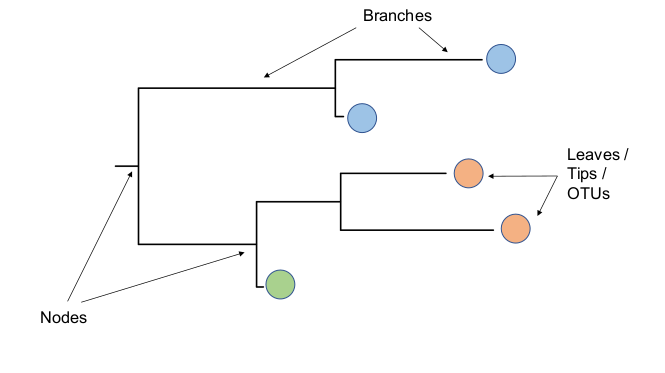
\includegraphics{img/basic-tree.png}
\caption{A phylogenetic tree}
\end{figure}

    \hypertarget{nodes}{%
\subsubsection{Nodes}\label{nodes}}

There are two types of \textit{nodes} in a phylogenetic tree; external
nodes, also called `tips' or `leaves' of the tree (i.e.~taxa), and
internal nodes which denote their hypothetical ancestors.

\hypertarget{branches}{%
\subsubsection{Branches}\label{branches}}

The \textit{branches} in a tree are shown as lines connecting the nodes.
They show the path of transmission of genetic information from one
generation to the next. Branch lengths indicate genetic change i.e.~the
longer the branch, the more genetic change (or divergence) has occurred.

\hypertarget{root}{%
\subsubsection{Root}\label{root}}

A phylogenetic tree can be unrooted or rooted as shown below.

    \begin{figure}
\centering
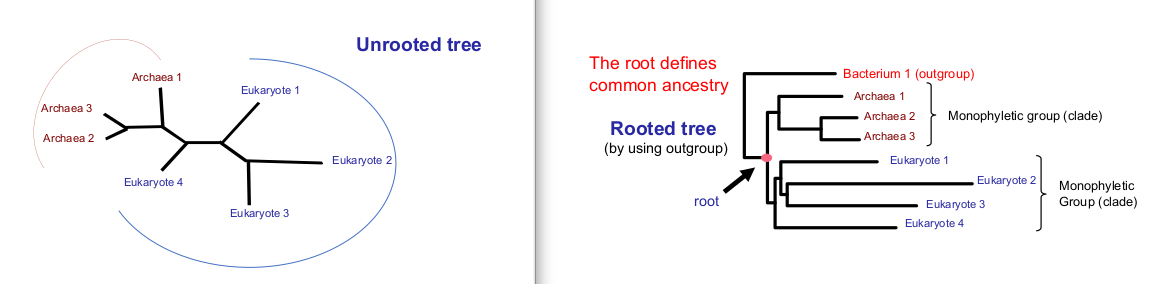
\includegraphics{img/unrooted_vs_rooted.png}
\caption{A phylogenetic tree}
\end{figure}

    The \textit{root} of a phylogenetic tree is the most recent common
ancestor of all of the taxa in the tree. It is therefore the oldest part
of the tree and tells us the direction of evolution, with the flow of
genetic information moving from the root, towards the tips with each
successive generation. Deciding upon an appropriate root position is
critical for phylogenetic interpretation because the root tells us the
direction of evolution and so affects statements that we make about
patterns of relatedness.

There are two main approaches that can be used to root a tree, midpoint
rooting and outgroup rooting. We will describe these approaches in more
detail later in the tutorial.

\hypertarget{topology}{%
\subsubsection{Topology}\label{topology}}

The \textit{topology} is the branching structure of the tree and the same
topology can be drawn in lots of different ways. It is of particular
biological significance because it indicates patterns of relatedness
among taxa, meaning that trees with the same topology and root have the
same biological interpretation.

    \hypertarget{microbial-phylogenetic-trees}{%
\subsection{Microbial phylogenetic
trees}\label{microbial-phylogenetic-trees}}

In the context of infectious diseases epidemiology, phylogenetic trees
are commonly used to define evolutionary relationships between strains
of the same bacterial species. This is possible because bacteria
reproduce clonally. During clonal reproduction, bacterial progenitor
cells replicate their DNA at high fidelity. Despite this, random errors
in DNA replication may still occur, resulting in a clonal progeny that
will inherit these genetic replication `errors' (i.e.~mutations) in
their DNA and may not be strictly identical to their progenitor cells.
Bacterial strains that have recently originated from the same progenitor
cell are thus expected to share identical genomes or have diverged at
most by only a few genetic differences (mutations). The number and
pattern of shared mutations between bacterial strains can be used to
reconstruct their genealogical and evolutionary relationships.

On a phylogenetic tree, isolated bacterial strains are depicted on the
\textit{leaves} of the tree, whereas the internal nodes of the tree denote
their hypothetical ancestors. Groups of bacterial strains (taxa) that
share the same common ancestor form a \textit{monophyletic} group (also
known as \textit{clade}). A group of strains that descends from a common
ancestor, but does not include all descendants, is called
\textit{paraphyletic}.

    \hypertarget{how-are-phylogenetic-trees-reconstructed}{%
\subsection{How are phylogenetic trees
reconstructed?}\label{how-are-phylogenetic-trees-reconstructed}}

Today almost all phylogenetic trees are inferred from molecular sequence
data, most often from DNA sequences. This is because DNA is an inherited
material; it can easily, reliably and inexpensively be extracted and
sequenced; and DNA sequences are highly specific to bacterial species
and strains.

The goal is to generate a multiple sequence alignment of the DNA
sequences of the bacterial species or strains and use this to
re-construct the phylogenetic tree. Polymorphic sites (that is,
nucleotide positions that are variable across multiple strains) in
multiple alignments are used to infer evolutionary relationships,
whereas monomorphic sites (nucleotide positions with the same DNA base)
are generally ignored. The figure below shows an example of a simple
multiple alignment of eight sites from four strains, which include
monomorphic (squared) and polymorphic sites. Genetic changes in the
phylogenetic tree are showed as coloured vertical rectangles on the
branch where they originated. The identification of genetic changes
(alleles) that are unique and common to multiple taxa (strains) are used
to group them into monophyletic groups (clades) in a hierarchical manner
with the goal of constructing the most plausible genealogical
relationships between strains and clades.

    \begin{figure}
\centering
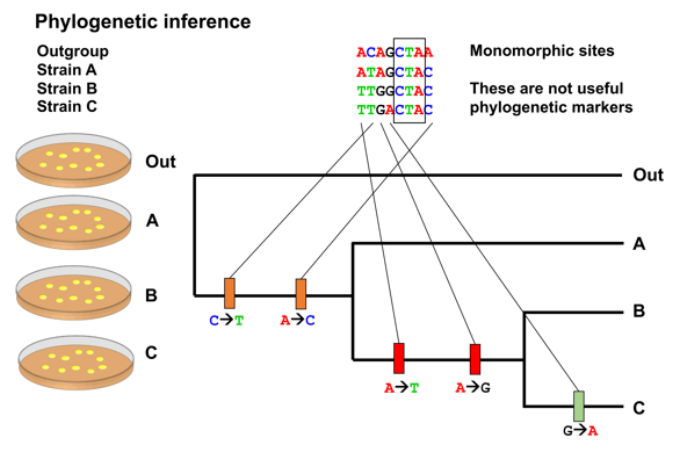
\includegraphics{img/phylogeny.png}
\caption{Overview of phylogeny construction}
\end{figure}

    There are many computational methods for reconstructing a tree from
sequence data, e.g.~Parsimony, Maximum Likelihood. Most methods require
a model of evolution (substitution model) to provide information on how
the sequences evolved. We won't expand on this here as it is beyond the
scope of this tutorial.

    \hypertarget{data-selection-for-phylogenies}{%
\subsection{Data selection for
phylogenies}\label{data-selection-for-phylogenies}}

The type of sequence data that is used to construct a phylogenetic tree
can vary. A tree can be constructed using sequence data from:

\begin{itemize}
\tightlist
\item
  a single gene
\item
  Multi-locus sequence typing (MLST) data: a set of housekeeping genes
  for a species
\item
  Core genome MLST (cgMLST) data: an expanded MLST scheme using all
  genes shared by all strains within a species
\item
  Whole genome MLST (wgMLST) data: an expanded cgMLST scheme to include
  a selection of accessory genes
\item
  entire genome reconstructed from the whole genome sequence data
\end{itemize}

The sequences to include and the type of data that you choose when
constructing your phylogenetic tree will depend on your objective.

    \hypertarget{exercises}{%
\subsection{Exercises}\label{exercises}}

Look at the following tree and answer the questions that follow:

    \begin{figure}
\centering
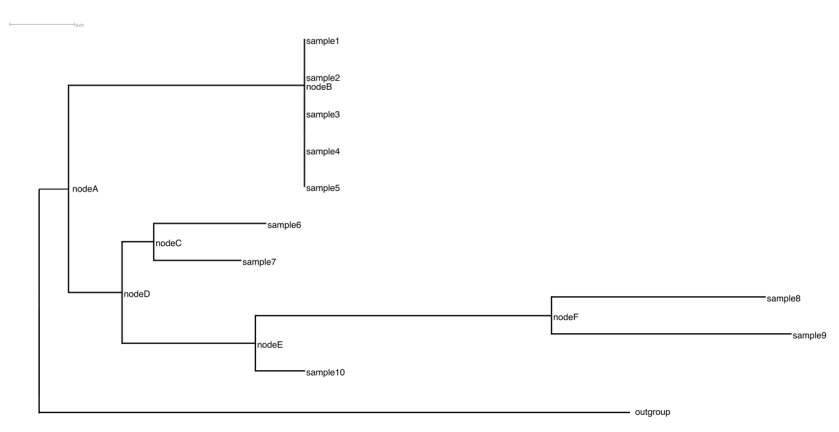
\includegraphics{img/test-tree.png}
\caption{Overview of phylogeny construction}
\end{figure}

    \begin{enumerate}
\def\labelenumi{\arabic{enumi}.}
\tightlist
\item
  How many nodes are in the tree?
\item
  What internal node corresponds to the most recent common ancestor of
  samples 8 and 10
\item
  Which term best describes a group that share the same common ancestor?
\end{enumerate}

\begin{enumerate}
\def\labelenumi{\alph{enumi}.}
\tightlist
\item
  Polyphyletic
\item
  Monophyletic
\item
  Paraphyletic
\end{enumerate}

    Now let's construct our first phylogeny: \href{gene.ipynb}{Phylogeny
from gene sequences}


    % Add a bibliography block to the postdoc



\newpage





    \hypertarget{phylogeny-from-gene-sequences}{%
\section{Phylogeny from gene
sequences}\label{phylogeny-from-gene-sequences}}

For our first phylogeny we will make a tree using the sequences of the
\textit{ompA} gene from 16 strains of \textit{C. trachomatis}. First, let's
check that you're in the right place. Type the command below in the
terminal window followed by the Enter key:

    \begin{tcolorbox}[breakable, size=fbox, boxrule=1pt, pad at break*=1mm,colback=cellbackground, colframe=cellborder]
\prompt{In}{incolor}{ }{\boxspacing}
\begin{Verbatim}[commandchars=\\\{\}]
\PY{n+nb}{pwd}
\end{Verbatim}
\end{tcolorbox}

    It should display something like:

\texttt{/home/manager/course\_data/snp\_phlogeny/data}

The gene sequences for the 16 strains are found in a multifasta file
called \texttt{ompA.fa} in the \texttt{gene} directory. These nucleotide
sequences have been constructed from sequence data of the 16 strains. We
won't cover how the genes were constructed here but will learn more
about this in a later tutorial.

Take a look at the file containing the gene sequences:

    \begin{tcolorbox}[breakable, size=fbox, boxrule=1pt, pad at break*=1mm,colback=cellbackground, colframe=cellborder]
\prompt{In}{incolor}{ }{\boxspacing}
\begin{Verbatim}[commandchars=\\\{\}]
\PY{n+nb}{cd}\PY{+w}{ }gene
\end{Verbatim}
\end{tcolorbox}

    \begin{tcolorbox}[breakable, size=fbox, boxrule=1pt, pad at break*=1mm,colback=cellbackground, colframe=cellborder]
\prompt{In}{incolor}{ }{\boxspacing}
\begin{Verbatim}[commandchars=\\\{\}]
cat\PY{+w}{ }ompA.fa
\end{Verbatim}
\end{tcolorbox}

    \hypertarget{introducing-the-dataset}{%
\subsection{Introducing the dataset}\label{introducing-the-dataset}}

The dataset used in this section has in part been derived from the
following paper:

\begin{quote}
\textbf{The Swedish new variant of Chlamydia trachomatis: genome
sequence, morphology, cell tropism and phenotypic characterization}\\
Unemo M, Seth-Smith HMB, Cutcliffe LT, Skilton RJ, Barlow D, Goulding D,
Persson K, Harris SR, Kelly A, Bjartling C, Fredlund H, Olcén P, Thomson
NR, Clarke IN. \textit{Microbiology 2010. doi: 10.1099/mic.0.036830-0}
PMID:
\href{https://www.ncbi.nlm.nih.gov/pmc/articles/PMC3541825/}{20093289}
\end{quote}

\textit{Chlamydia trachomatis} is one of the most prevalent human
pathogens in the world, causing a variety of infections. It is the
leading cause of sexually transmitted infections (STIs), with an
estimated 131 million new cases each year. Additionally, it is also the
leading cause of preventable infectious blindness with tens of millions
of people thought to have active disease.

Historically, the most commonly used tool for typing \textit{C.
trachomatis} isolates was serotyping using the MOMP (major outer
membrane protein), which is encoded by the \textit{ompA} gene. There are
two biovars of C. trachomatis:

\begin{itemize}
\tightlist
\item
  the \textit{trachoma} biovar includes ocular and urogenital strains,
  which cause the majority of trachoma and STIs, and are characterised
  by localised infections of the epithelial surface of the conjunctiva
  or genital mucosa;
\item
  the \textit{lymphogranuloma venereum (LGV)} biovar includes strains
  which are distinguished by their ability to spread systemically
  thorough the lymphatic system, causing genital ulceration and bubonic
  disease.
\end{itemize}

Based on MOMP serotyping, \textit{C. trachomatis} has been subdivided into
between 15 and 19 serotypes: the \textit{trachoma} biovar includes ocular
serotypes A to C and urogenital serotypes D to K, while the \textit{LGV}
biovar includes serotypes L1, L2 (including L2a, b and c) and L3.

In 2006, a new variant of \textit{C. trachomatis}, known as NV was
reported in Sweden and triggered a European health alert. During this
time it became the dominant strain circulating in some European
countries and began to spread world wide. The reason for this was that
it evaded detection by the widely used PCR-based diagnostic test. During
this exercise we will place this New Variant of \textit{C. trachomatis}
(NV) in the context of several other \textit{C.trachomatis} strains based
on the ompA gene.

    \hypertarget{viewing-the-alignment-in-seaview}{%
\subsection{Viewing the alignment in
Seaview}\label{viewing-the-alignment-in-seaview}}

To view our gene sequences and produce a phylogeny we will use a program
called \texttt{Seaview}. \texttt{Seaview} is a graphical user interface
(GUI) that combines a number of the most popular alignment and phylogeny
programs. Launch \texttt{Seaview}

    \begin{tcolorbox}[breakable, size=fbox, boxrule=1pt, pad at break*=1mm,colback=cellbackground, colframe=cellborder]
\prompt{In}{incolor}{ }{\boxspacing}
\begin{Verbatim}[commandchars=\\\{\}]
seaview\PY{+w}{ }\PY{p}{\PYZam{}}
\end{Verbatim}
\end{tcolorbox}

    Now load the file \texttt{ompA.fa} by selecting `File' and `Open' from
the main menu.

    \begin{figure}
\centering
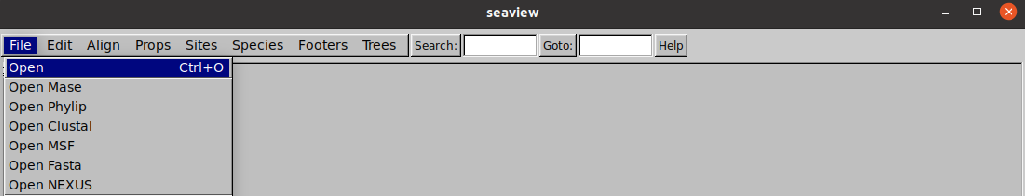
\includegraphics{img/seaview_1.png}
\caption{Seaview}
\end{figure}

    \begin{figure}
\centering
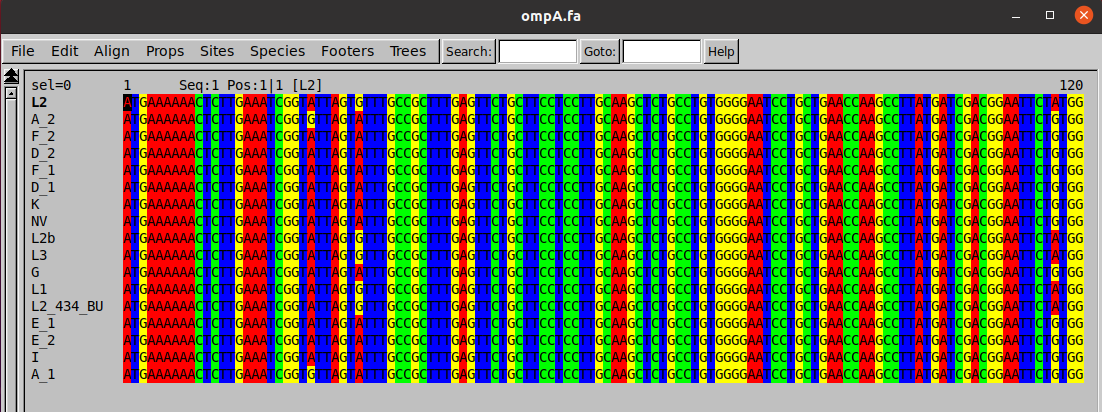
\includegraphics{img/seaview_2.png}
\caption{ompA alignment in Seaview}
\end{figure}

    \hypertarget{multiple-sequence-alignment}{%
\subsection{Multiple sequence
alignment}\label{multiple-sequence-alignment}}

Homology among DNA, RNA, or proteins is typically inferred from their
nucleotide or amino acid sequence similarity. Significant similarity is
strong evidence that two sequences are related by evolutionary changes
from a common ancestral sequence. Alignments of multiple sequences are
used to indicate which regions of each sequence are homologous.

Therefore before we perform any phylogenetic analysis, we must make sure
that the columns in our data represent homologous bases. With gene or
protein sequence data, this usually means aligning the nucleotide or
amino acid sequences using a multiple alignment program. Length
differences of the sequences complicate multiple sequence alignment
because these require the insertion of gaps into an alignment to ensure
that homologous sites remain aligned. When possible, alignments should
be checked by eye.

\texttt{Seaview} allows alignment using two programs, \texttt{clustal}
and \texttt{muscle}. Generally \texttt{muscle} is faster, providing
protein alignments that are of similar quality to \texttt{clustal}. It
is usually better to align genes after translating them into amino
acids, so we will do that here.

    On the `Props' menu tick `View as proteins'.

    \begin{figure}
\centering
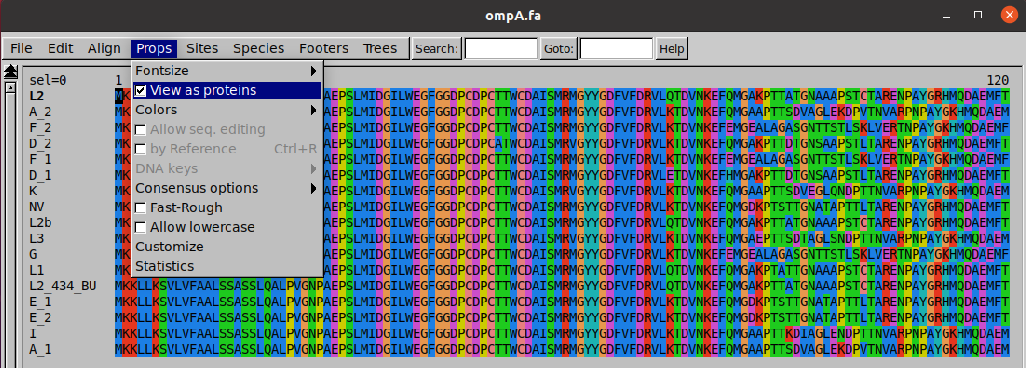
\includegraphics{img/seaview_3.png}
\caption{View as proteins in Seaview}
\end{figure}

    To run the alignment, select `Align' then `Align all' from the main
menu.

    \begin{figure}
\centering
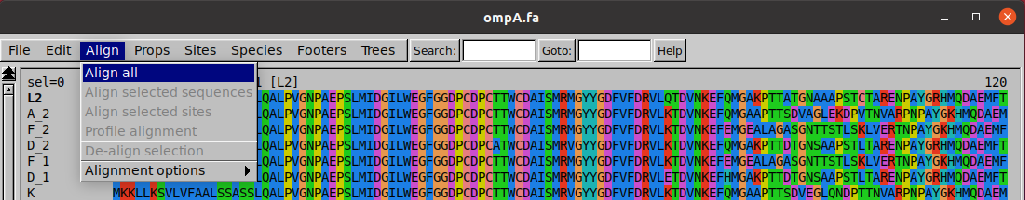
\includegraphics{img/seaview_4.png}
\caption{Aign all proteins in Seaview}
\end{figure}

    When the alignment process is complete, \texttt{Seaview} will have
inserted gaps into the sequences so that homologous sites (or at least
homologous according to the alignment program) are lined up in columns.
Look at the alignment, it should now be clearer how the sequences differ
from one another.

    \begin{figure}
\centering
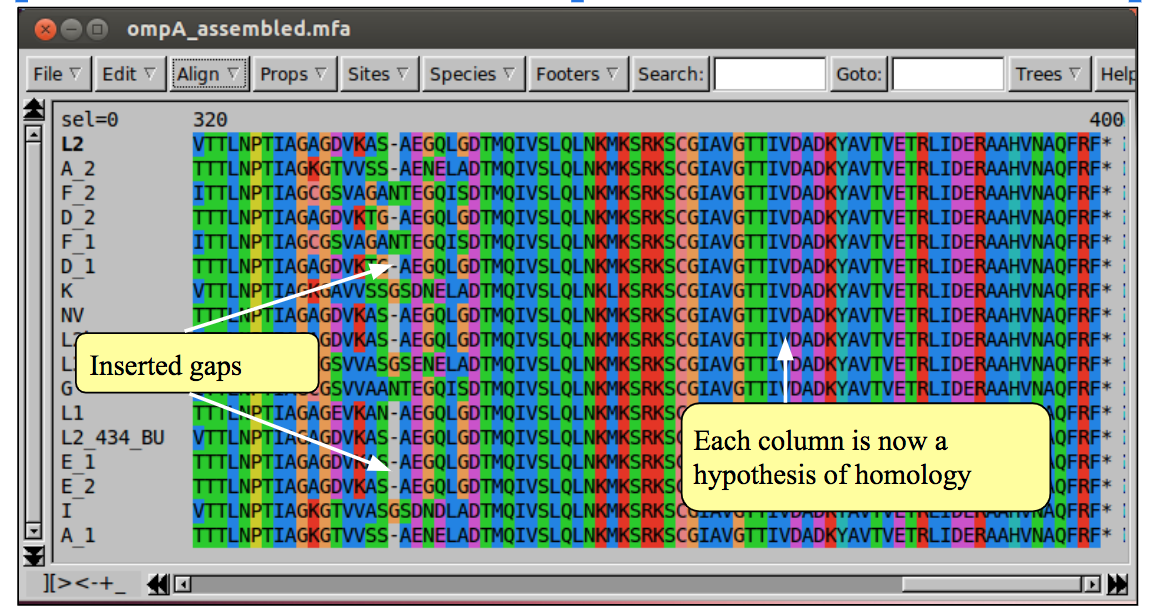
\includegraphics{img/seaview_5.png}
\caption{Protein alignment in Seaview}
\end{figure}

    Now turn off protein view and you will see that the nucleotides are also
now aligned.

    \begin{figure}
\centering
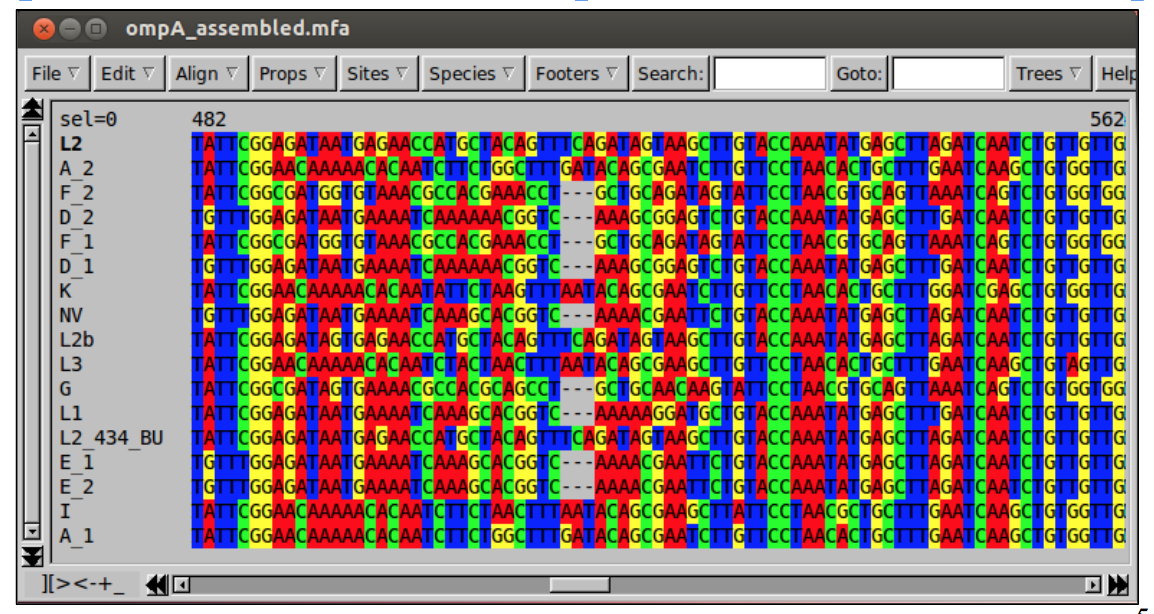
\includegraphics{img/seaview_6.png}
\caption{Nucleotide alignment in Seaview}
\end{figure}

    \hypertarget{phylogeny-estimation-using-phyml}{%
\subsection{Phylogeny estimation using
PhyML}\label{phylogeny-estimation-using-phyml}}

To estimate the phylogeny, we will use a program called \texttt{PhyML},
which is included in \texttt{Seaview}. \texttt{PhyML} uses a maximum
likelihood (ML) method to estimate the tree and includes a number of
nucleotide substitution models ranging from the very simple (and could
be unrealistic) to more complex ones. Evolutionary (or substitution)
models are statistical models that describe the substitution and
divergence of sequences over time.

To create a tree in \texttt{Seaview}, select `Trees' and `PhyML' from
the main menu.

    \begin{figure}
\centering
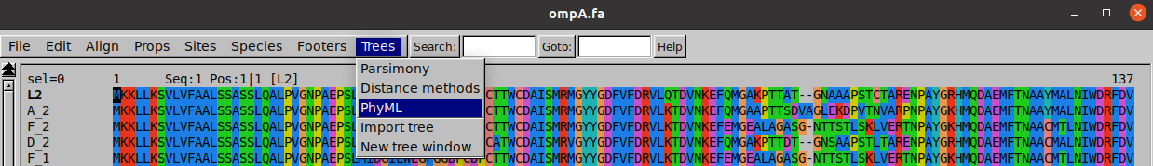
\includegraphics{img/phyml.png}
\caption{Creating a treee with PhyML}
\end{figure}

    Choose the \textit{GTR} (General Time Reversible) model for substitution
rates, set all other parameters as shown below and click \texttt{Run}.

    \begin{figure}
\centering
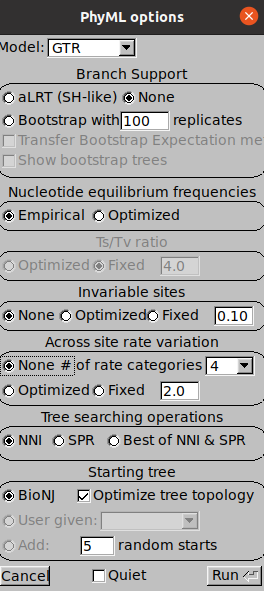
\includegraphics{img/tree_settings.png}
\caption{Tree Settings}
\end{figure}

    Once the run has finished, click `OK' and you should see a phylogenetic
tree as shown below. The tree created by \texttt{PhyML} includes the
topology of tree (i.e., the relationships between sequences) and the
branch lengths (i.e., the amount of change occurring in each lineage).
Therefore, the tree is drawn as a \textit{phylogram}, in which the length
of branches is proportional to the amount of evolutionary change.

    \begin{figure}
\centering
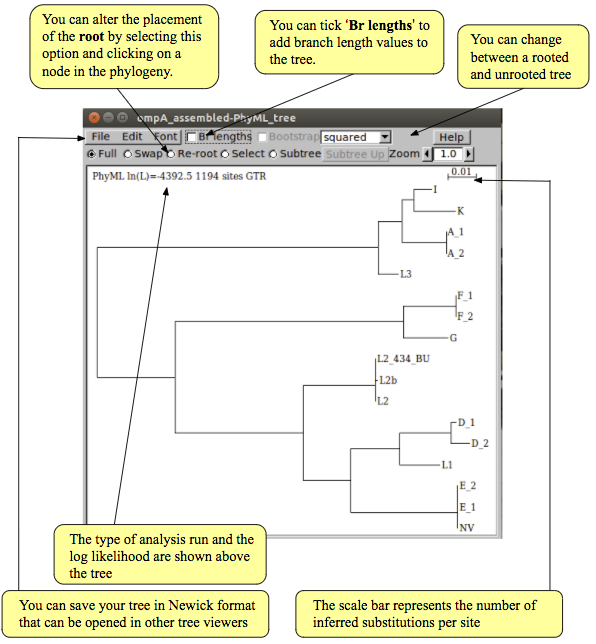
\includegraphics{img/tree_with_descriptions.png}
\caption{Phylogenetic tree of ompA gene with detailed description}
\end{figure}

    \hypertarget{phylogeny-estimation-with-bootstrapping}{%
\subsection{Phylogeny estimation with
bootstrapping}\label{phylogeny-estimation-with-bootstrapping}}

Bootstrapping is a statistical technique to assess the confidence level
around each phylogenetic node. The bootstrapping values indicates how
many times out of 100, the same branch was observed when repeating the
phylogenetic reconstruction on a re-sampled set of the data. Robust
relationship should be repeatable, and subsequently observed in a large
proportion of randomised data. Therefore, if you get 100 out of 100
times for a particular node, you can be more confident that the observed
branch is not due to chance, but likely to be real.

To estimate a bootstrapped phylogeny for the \textit{ompA} data, start by
creating a new phylogeny as before and then click on `Bootstrap' in the
`Branch Support' box, and enter `10' in the replicates box. The
processing of the 10 replicates may take a few minutes, so you could
move on while this is running. Ideally you would run more replicates
(100 or 1000), but to save time we will only run 10 replicates here.

    \begin{figure}
\centering
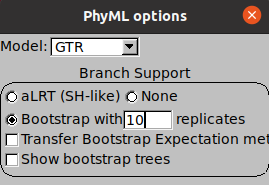
\includegraphics{img/bootstrap.png}
\caption{Bootstrapping option}
\end{figure}

    Once the search is complete, you can show the bootstrap values on the
tree by ticking the \textbf{Br support} box.

    \begin{figure}
\centering
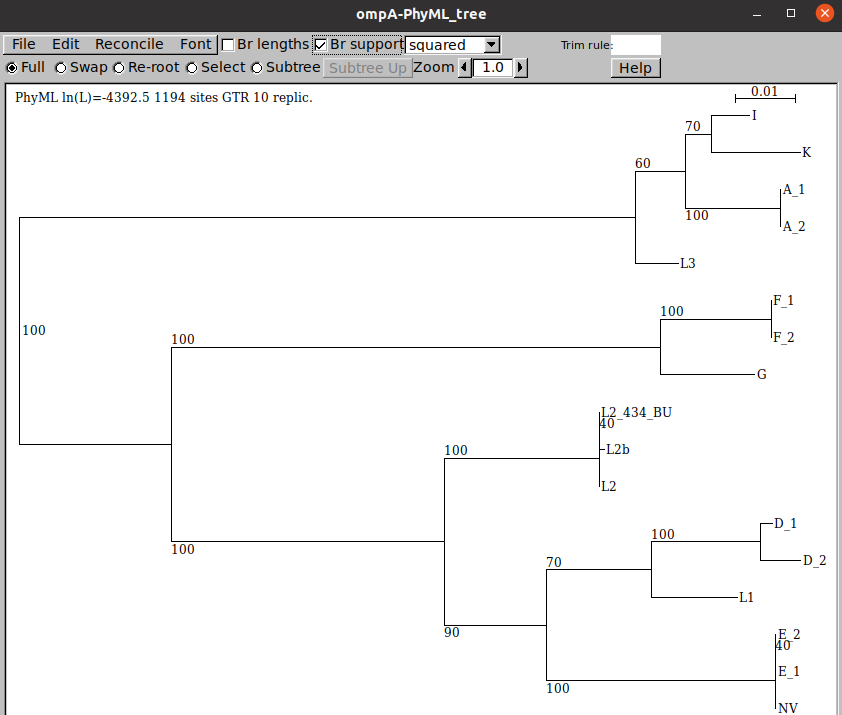
\includegraphics{img/tree_with_bootstraps.png}
\caption{Phylogenetic tree with bootstraps}
\end{figure}

    Each node in the tree now has an associated value out of 100, its
bootstrap. Can you identify any nodes that are not robust? Unfortunately
there is no generally accepted threshold for significant bootstrap
robustness, so you must use your judgement.

\textbf{WARNING!:} bootstrap proportions are measures of robustness, or
repeatability. A high bootstrap value indicates that a given node tends
to occur in every analysis. This does not guarantee that the node is
correct. For example, if the substitution model is inaccurate, it could
produce the wrong answer in every estimation.

    \hypertarget{phylogeny-visualisation}{%
\subsection{Phylogeny visualisation}\label{phylogeny-visualisation}}

In addition to \texttt{Seaview} there are many other tools that can be
used to visualise phylogenetic trees including \texttt{FigTree},
\texttt{Microreact} and \texttt{iToL}. As a short exercise, let's use
\texttt{FigTree} to visualise our tree. \texttt{FigTree} is more
versatile than the tree viewer in \texttt{Seaview}, allowing you to
colour branches and taxa, redraw the tree in a number of ways and output
the results in a large number of graphics formats including \texttt{eps}
and \texttt{pdf}. It is particularly useful for preparing figures for
manuscripts.

First, export the tree produced by PhyML by choosing the `File' and Save
unrooted tree' from the main menu. The file will be saved in newick
format. A newick file is a standard text-based format for representing
trees in computer-readable form using (nested) parentheses and commas.

Open FigTree by typing `figtree' in the terminal.

    \begin{tcolorbox}[breakable, size=fbox, boxrule=1pt, pad at break*=1mm,colback=cellbackground, colframe=cellborder]
\prompt{In}{incolor}{ }{\boxspacing}
\begin{Verbatim}[commandchars=\\\{\}]
figtree\PY{+w}{ }\PY{p}{\PYZam{}}
\end{Verbatim}
\end{tcolorbox}

    Now open the exported newick tree file using \texttt{FigTree}.

    \begin{figure}
\centering
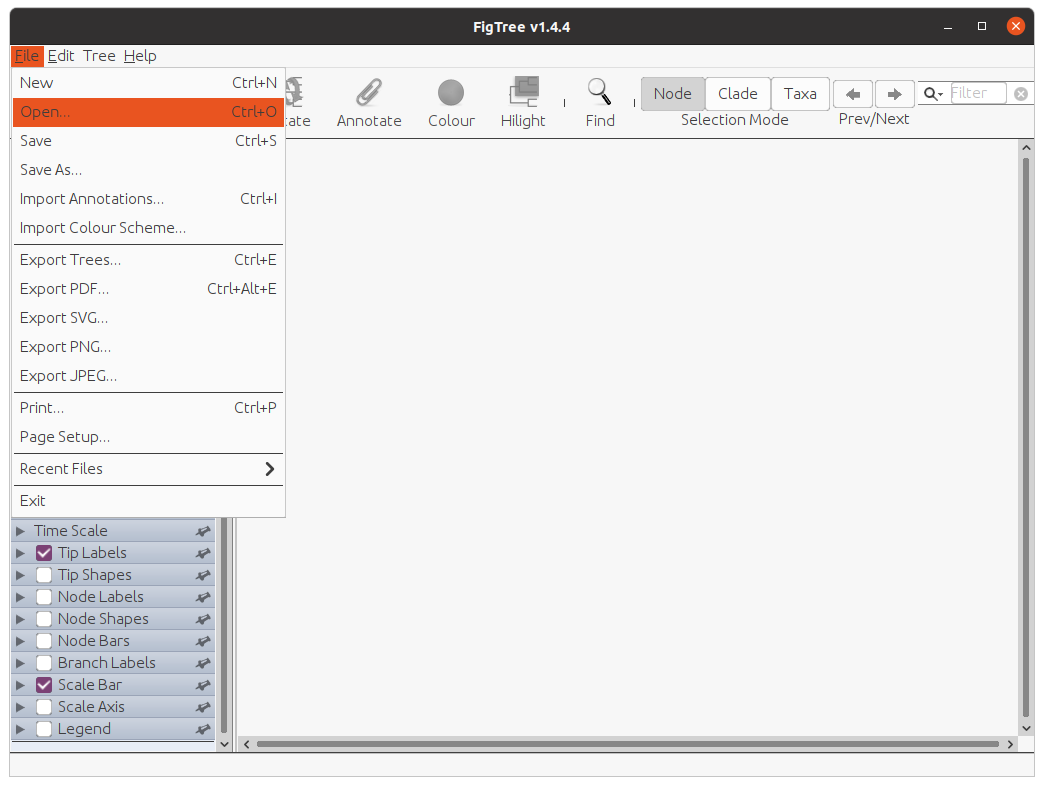
\includegraphics{img/figtree.png}
\caption{Open newick file with FigTree}
\end{figure}

    If you have time explore the different functionality available in
\texttt{FigTree}.

    \begin{figure}
\centering
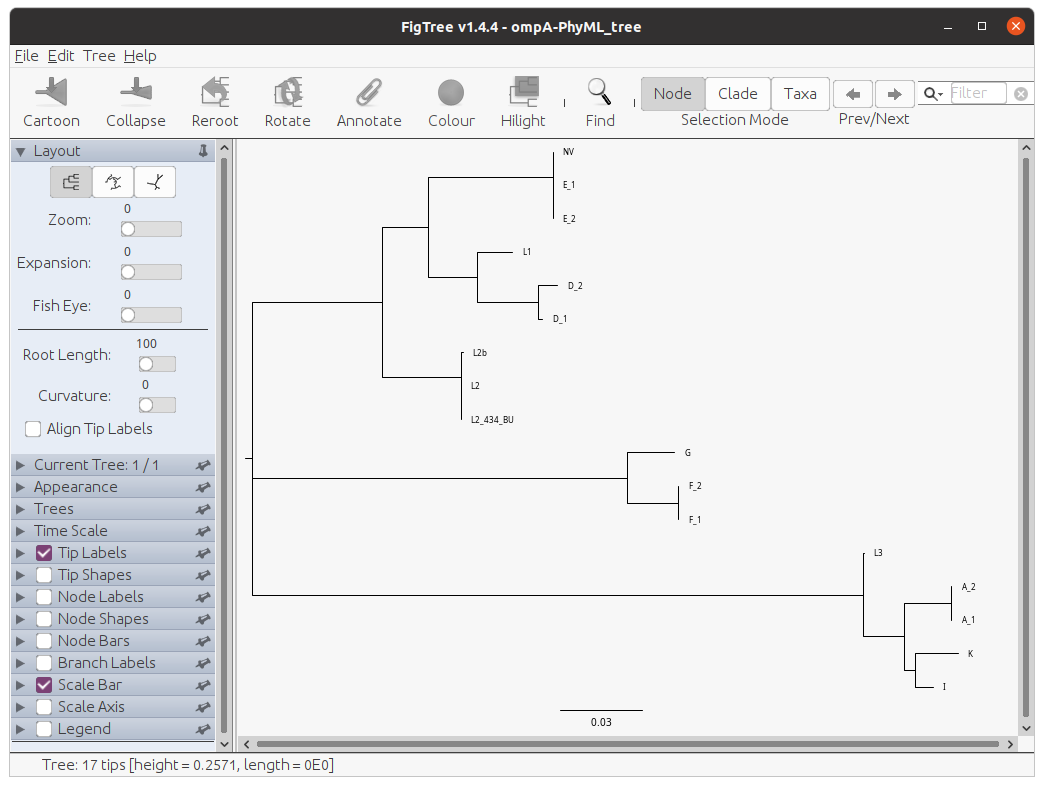
\includegraphics{img/tree_in_figtree.png}
\caption{Open newick file with FigTree}
\end{figure}

    \hypertarget{exercises}{%
\subsection{Exercises}\label{exercises}}

\begin{enumerate}
\def\labelenumi{\arabic{enumi}.}
\tightlist
\item
  From the trees that you have produced, which MOMP type would you
  suggest the new variant (NV) strain belongs to?
\item
  Do the ompA trees agree with the separation of \textit{C. trachomatis}
  into trachoma (serotypes A to K) and LGV (L serotypes) biovars?
\end{enumerate}

    Now move on to the next section: \href{snp_phylogeny.ipynb}{Constructing
phylogeny from whole genome sequence data}


    % Add a bibliography block to the postdoc



\newpage





    \hypertarget{phylogeny-from-whole-genome-sequence-data}{%
\section{Phylogeny from whole genome sequence
data}\label{phylogeny-from-whole-genome-sequence-data}}

    When we sequence a population, we aim to capture the variation (SNPs,
indels, gene gain and loss etc.) in the samples and use it to infer the
relationships between the samples. Two of the main approaches to
capturing this variation and reconstructing the bacterial genomes are:

\begin{itemize}
\tightlist
\item
  De novo genome assembly and annotation
\item
  Mapping and variant calling against a reference genome
\end{itemize}

Each approach has it's benefits and limitations. We will focus on
mapping and variant calling in this tutorial. For mapping and variant
calling, whether we are dealing with different bacterial isolates, with
viral populations in a patient, or even with genomes of different human
individuals, the principles are essentially the same. Instead of
assembling the newly generated sequence reads de novo to produce a new
genome sequence, it is easier and much faster to align or map the
sequence reads to a reference genome. We can then readily identify SNPs
and indels that distinguish closely related populations or individual
organisms and may thus learn about genetic differences that may cause
drug resistance or increased virulence in pathogens, or changed
susceptibility to disease in humans. One important prerequisite for the
mapping of sequence data to work is that the reference and the
re-sequenced subject have the same genome architecture.

In this exercise, we will use sequence data from \textit{Salmonella
enterica serovar Typhi} samples to demonstrate the mapping and variant
calling approach. Importantly, although the data is based on real
sequence data, it has been edited to make it run more efficiently for
the purpose of this tutorial.

Navigate to the directory that contains the sequence data:

    \begin{tcolorbox}[breakable, size=fbox, boxrule=1pt, pad at break*=1mm,colback=cellbackground, colframe=cellborder]
\prompt{In}{incolor}{ }{\boxspacing}
\begin{Verbatim}[commandchars=\\\{\}]
\PY{n+nb}{cd}\PY{+w}{ }\PYZti{}/course\PYZus{}data/snp\PYZus{}phylogeny/data/typhi
\end{Verbatim}
\end{tcolorbox}

    Take a look at the directory containing the sequence data for the
samples:

    \begin{tcolorbox}[breakable, size=fbox, boxrule=1pt, pad at break*=1mm,colback=cellbackground, colframe=cellborder]
\prompt{In}{incolor}{ }{\boxspacing}
\begin{Verbatim}[commandchars=\\\{\}]
ls\PY{+w}{ }fastq
\end{Verbatim}
\end{tcolorbox}

    \hypertarget{introducing-the-tutorial-dataset}{%
\subsection{Introducing the tutorial
dataset}\label{introducing-the-tutorial-dataset}}

We will use data adapted from the following paper:

\begin{quote}
\textbf{A genomic snapshot of Salmonella enterica serovar Typhi in
Colombia}\\
Guevara, Paula Diaz, et al.\\
\textit{PLoS Neglected Tropical Diseases2021. doi:
10.1371/journal.pntd.0009755}\\
PMID:
\href{https://www.ncbi.nlm.nih.gov/pmc/articles/PMC8478212/}{34529660}
\end{quote}

\textit{Salmonella enterica serovar Typhi} (\textit{S. Typhi}) is the
causative agent of typhoid fever, with between 9--13 million cases and
116,800 associated deaths annually. Typhoid fever is still a public
health problem in many countries, including in Latin America, which has
a modelled incidence of up to 169 (32--642) cases per 100,000
person-years. Several international studies have aimed to fill data gaps
regarding the global distribution and genetic landscape of typhoid;
however, in spite of these efforts Latin America is still
underrepresented. This study provided the first enhanced insights into
the molecular epidemiology of S. Typhi in Colombia, using whole genome
sequencing data to investigate the population structure in Colombia and
identify predominant circulating genotypes.

    \hypertarget{overview-of-mapping-and-variant-calling-approach}{%
\subsection{Overview of mapping and variant calling
approach}\label{overview-of-mapping-and-variant-calling-approach}}

The diagram below illustrates the steps involved when mapping and
calling variants for a set of bacterial samples.

    \begin{tcolorbox}[breakable, size=fbox, boxrule=1pt, pad at break*=1mm,colback=cellbackground, colframe=cellborder]
\prompt{In}{incolor}{ }{\boxspacing}
\begin{Verbatim}[commandchars=\\\{\}]
!\PY{o}{[}Approach\PY{o}{]}\PY{o}{(}img/snp\PYZhy{}phylogeny\PYZhy{}approach.png\PY{o}{)}
\end{Verbatim}
\end{tcolorbox}

    The first step once you have obtained your sequence data (FASTQ) is to
QC the data. After QC, the sequence data is matched or aligned to a
reference genome (FASTA) in a process called read mapping to produce a
set of read aligments (SAM/BAM). These read alignments are inspected to
identify differences between the aligned reads and the reference genome.
This process is called variant calling and produces VCF files. In fact
during this process we capture information about every position in the
genome (variant and non-variant sites) in the VCFs. Each site in the VCF
has a set of quality filters applied and any sites identified as low
quaility (e.g.~less than 4 reads aligned at that position) are marked as
low quality in the VCF to produce a filtered VCF. We use this filtered
VCF file in a process called consensus caling to reconstruct a consensus
\textit{pseudosequence} or \textit{pseudogenome} for our sample (FASTA). In
the \textit{pseudogenome}, any sites marked as low quality will be
represented as an N in the reconstructed sequence. These pseudogenomes
(multi-FASTA) are then aligned and variation identified and used to
reconstruct a phylogeny of our samples.

    \hypertarget{exercise}{%
\subsection{Exercise}\label{exercise}}

Now let's analyse some data!

\hypertarget{prepare-the-data}{%
\subsubsection{Prepare the data}\label{prepare-the-data}}

First take a look at the sequence data provided.

    \begin{tcolorbox}[breakable, size=fbox, boxrule=1pt, pad at break*=1mm,colback=cellbackground, colframe=cellborder]
\prompt{In}{incolor}{ }{\boxspacing}
\begin{Verbatim}[commandchars=\\\{\}]
ls\PY{+w}{ }fastq/
\end{Verbatim}
\end{tcolorbox}

    \hypertarget{check-your-understanding}{%
\paragraph{Check your understanding}\label{check-your-understanding}}

\begin{enumerate}
\def\labelenumi{\arabic{enumi}.}
\tightlist
\item
  How many samples have been sequenced?
\item
  How many fastq files are there?
\end{enumerate}

    We will use the chromosome sequence of \textit{Salmonella typhi CT18} as
the reference genome. This has already been downloaded from RefSeq. Take
a look at the reference genome:

    \begin{tcolorbox}[breakable, size=fbox, boxrule=1pt, pad at break*=1mm,colback=cellbackground, colframe=cellborder]
\prompt{In}{incolor}{ }{\boxspacing}
\begin{Verbatim}[commandchars=\\\{\}]
ls\PY{+w}{ }ref/
\end{Verbatim}
\end{tcolorbox}

    Check the size of the reference file:

    \begin{tcolorbox}[breakable, size=fbox, boxrule=1pt, pad at break*=1mm,colback=cellbackground, colframe=cellborder]
\prompt{In}{incolor}{ }{\boxspacing}
\begin{Verbatim}[commandchars=\\\{\}]
assembly\PYZhy{}stats\PY{+w}{ }ref/Styphi\PYZus{}CT18.fa
\end{Verbatim}
\end{tcolorbox}

    Now use bwa to index the reference genome. This creates a lookup table
that bwa uses when matching the sequence reads against the reference
genome.

    \begin{tcolorbox}[breakable, size=fbox, boxrule=1pt, pad at break*=1mm,colback=cellbackground, colframe=cellborder]
\prompt{In}{incolor}{ }{\boxspacing}
\begin{Verbatim}[commandchars=\\\{\}]
bwa\PY{+w}{ }index\PY{+w}{ }ref/Styphi\PYZus{}CT18.fa
\end{Verbatim}
\end{tcolorbox}

    \hypertarget{check-your-understanding}{%
\paragraph{Check your understanding}\label{check-your-understanding}}

\begin{enumerate}
\def\labelenumi{\arabic{enumi}.}
\setcounter{enumi}{2}
\tightlist
\item
  How many sequences in the reference fasta file?
\item
  What are the names of the sequences in the reference fasta file?
\item
  What is the size of the reference?
\item
  What additional files did the indexing step produce?
\end{enumerate}

    \hypertarget{qc-the-sequence-data}{%
\subsubsection{QC the sequence data}\label{qc-the-sequence-data}}

An important first step in any analysis is QC of the data. We will the
FastQC software to QC the data. First create a directory for the qc
results:

    \begin{tcolorbox}[breakable, size=fbox, boxrule=1pt, pad at break*=1mm,colback=cellbackground, colframe=cellborder]
\prompt{In}{incolor}{ }{\boxspacing}
\begin{Verbatim}[commandchars=\\\{\}]
\PY{n+nb}{cd}\PY{+w}{ }fastq
mkdir\PY{+w}{ }qc\PYZus{}results
\end{Verbatim}
\end{tcolorbox}

    Run FastQC on the all the fastq files and store the results in the
directory \texttt{qc\_results}:

    \begin{tcolorbox}[breakable, size=fbox, boxrule=1pt, pad at break*=1mm,colback=cellbackground, colframe=cellborder]
\prompt{In}{incolor}{ }{\boxspacing}
\begin{Verbatim}[commandchars=\\\{\}]
fastqc\PY{+w}{ }\PYZhy{}o\PY{+w}{ }qc\PYZus{}results\PY{+w}{ }*.fastq.gz
\end{Verbatim}
\end{tcolorbox}

    This will create one html report for each of the fastq files. Take a
look:

    \begin{tcolorbox}[breakable, size=fbox, boxrule=1pt, pad at break*=1mm,colback=cellbackground, colframe=cellborder]
\prompt{In}{incolor}{ }{\boxspacing}
\begin{Verbatim}[commandchars=\\\{\}]
ls\PY{+w}{ }qc\PYZus{}results/
\end{Verbatim}
\end{tcolorbox}

    If we have lots of samples it will be difficult to manually inspect each
file. Therefore we will use multiQC to collate all the QC reports into
one file.

    \begin{tcolorbox}[breakable, size=fbox, boxrule=1pt, pad at break*=1mm,colback=cellbackground, colframe=cellborder]
\prompt{In}{incolor}{ }{\boxspacing}
\begin{Verbatim}[commandchars=\\\{\}]
multiqc\PY{+w}{ }qc\PYZus{}results
\end{Verbatim}
\end{tcolorbox}

    Open the collated report \texttt{multiqc\_report.html} in firefox.

    \begin{tcolorbox}[breakable, size=fbox, boxrule=1pt, pad at break*=1mm,colback=cellbackground, colframe=cellborder]
\prompt{In}{incolor}{ }{\boxspacing}
\begin{Verbatim}[commandchars=\\\{\}]
firefox\PY{+w}{ }multiqc\PYZus{}report.html\PY{+w}{ }\PY{p}{\PYZam{}}
\end{Verbatim}
\end{tcolorbox}

    \begin{figure}
\centering
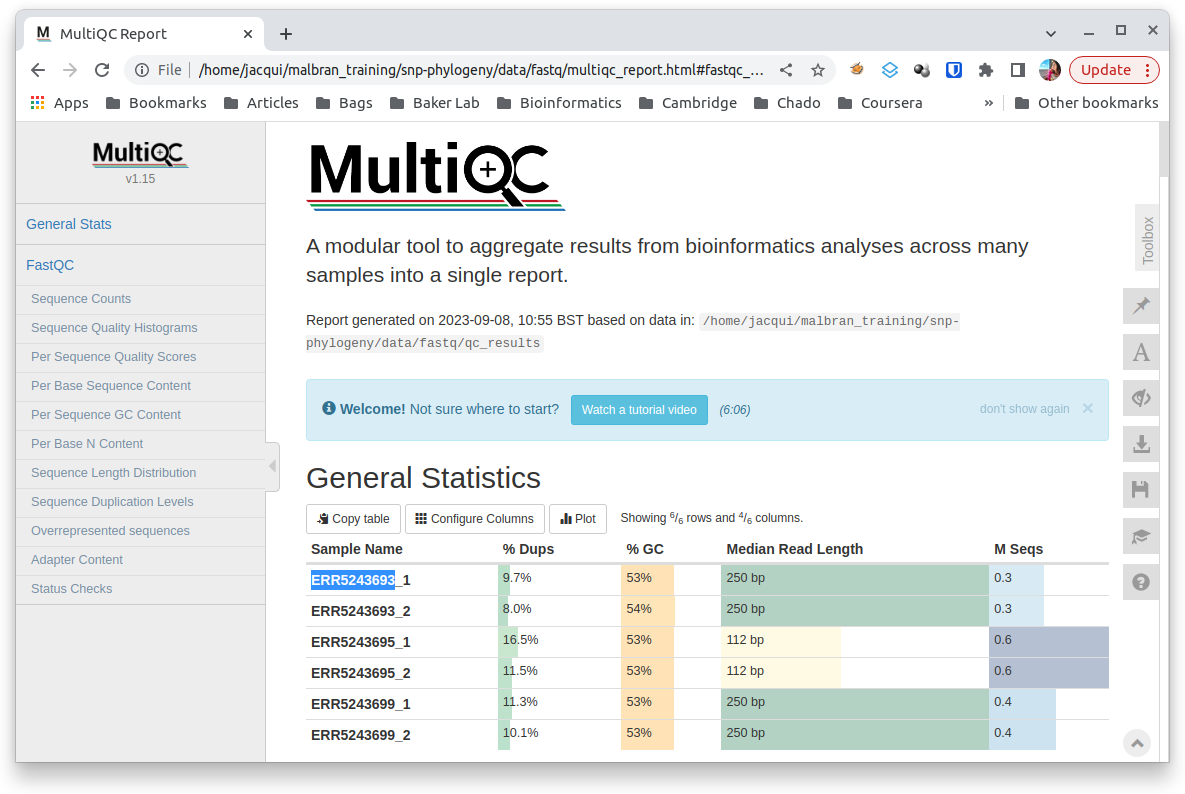
\includegraphics{img/multiqc.png}
\caption{MultiQC results}
\end{figure}

    \hypertarget{check-your-understanding}{%
\paragraph{Check your understanding}\label{check-your-understanding}}

\begin{enumerate}
\def\labelenumi{\arabic{enumi}.}
\tightlist
\item
  What is the median read length for sample ERR5243693?
\item
  Which sample has the largest yield (most sequence data)?
\end{enumerate}

    \hypertarget{trim-the-reads-to-remove-low-quality-and-adapter-sequence}{%
\subsubsection{Trim the reads to remove low quality and adapter
sequence}\label{trim-the-reads-to-remove-low-quality-and-adapter-sequence}}

If your sequence reads have a high level of adapter contamination and/or
have low quality bases at the end of the reads you can trim the reads to
remove these sequences. There are several software that can be used to
do this including trimmomatic and fastp.

Use fastp to trim the reads for sample ERR5243693.

    \begin{tcolorbox}[breakable, size=fbox, boxrule=1pt, pad at break*=1mm,colback=cellbackground, colframe=cellborder]
\prompt{In}{incolor}{ }{\boxspacing}
\begin{Verbatim}[commandchars=\\\{\}]
fastp\PY{+w}{ }\PY{l+s+se}{\PYZbs{}}
\PY{+w}{   }\PYZhy{}\PYZhy{}in1\PY{+w}{ }ERR5243693\PYZus{}1.fastq.gz\PY{+w}{ }\PYZhy{}\PYZhy{}in2\PY{+w}{ }ERR5243693\PYZus{}2.fastq.gz\PY{+w}{ }\PY{l+s+se}{\PYZbs{}}
\PY{+w}{   }\PYZhy{}\PYZhy{}out1\PY{+w}{ }ERR5243693\PYZus{}1.trim.fastq.gz\PY{+w}{ }\PY{l+s+se}{\PYZbs{}}
\PY{+w}{   }\PYZhy{}\PYZhy{}out2\PY{+w}{ }ERR5243693\PYZus{}2.trim.fastq.gz\PY{+w}{ }\PY{l+s+se}{\PYZbs{}}
\PY{+w}{   }\PYZhy{}\PYZhy{}json\PY{+w}{ }ERR5243693.fastp.json\PY{+w}{ }\PYZhy{}\PYZhy{}html\PY{+w}{ }ERR5243693.fastp.html\PY{+w}{ }\PY{l+s+se}{\PYZbs{}}
\PY{+w}{   }\PYZhy{}\PYZhy{}detect\PYZus{}adapter\PYZus{}for\PYZus{}pe\PY{+w}{ }\PYZhy{}\PYZhy{}cut\PYZus{}mean\PYZus{}quality\PY{+w}{ }\PY{l+m}{20}\PY{+w}{ }\PY{l+s+se}{\PYZbs{}}
\PY{+w}{   }\PYZhy{}\PYZhy{}thread\PY{+w}{ }\PY{l+m}{2}
\end{Verbatim}
\end{tcolorbox}

    Now repeat for the other samples and look at the output from fastp:

    \begin{tcolorbox}[breakable, size=fbox, boxrule=1pt, pad at break*=1mm,colback=cellbackground, colframe=cellborder]
\prompt{In}{incolor}{ }{\boxspacing}
\begin{Verbatim}[commandchars=\\\{\}]
head\PY{+w}{ }\PYZhy{}20\PY{+w}{ }ERR5243693.fastp.json
head\PY{+w}{ }\PYZhy{}20\PY{+w}{ }ERR5243695.fastp.json
head\PY{+w}{ }\PYZhy{}20\PY{+w}{ }ERR5243699.fastp.json
\end{Verbatim}
\end{tcolorbox}

    \hypertarget{check-your-understanding}{%
\paragraph{Check your understanding}\label{check-your-understanding}}

\begin{enumerate}
\def\labelenumi{\arabic{enumi}.}
\tightlist
\item
  How much data (bp/base pairs) was lost due to trimming and adapter
  removal?
\end{enumerate}

    \hypertarget{map-the-data-to-a-reference-genome}{%
\subsubsection{Map the data to a reference
genome}\label{map-the-data-to-a-reference-genome}}

    When performing any data analysis it is good practice to arrange your
data in a logical way rather than putting all files in a single
directory. Let's create a directory to store the results of mapping the
reads to the reference genome:

    \begin{tcolorbox}[breakable, size=fbox, boxrule=1pt, pad at break*=1mm,colback=cellbackground, colframe=cellborder]
\prompt{In}{incolor}{ }{\boxspacing}
\begin{Verbatim}[commandchars=\\\{\}]
mkdir\PY{+w}{ }../samtools
\PY{n+nb}{cd}\PY{+w}{ }../samtools
\end{Verbatim}
\end{tcolorbox}

    Use \texttt{bwa} to map the reads for sample ERR5243693 to the reference
genome.

    \begin{tcolorbox}[breakable, size=fbox, boxrule=1pt, pad at break*=1mm,colback=cellbackground, colframe=cellborder]
\prompt{In}{incolor}{ }{\boxspacing}
\begin{Verbatim}[commandchars=\\\{\}]
bwa\PY{+w}{ }mem\PY{+w}{ }\PYZhy{}t\PY{+w}{ }\PY{l+m}{2}\PY{+w}{ }../ref/Styphi\PYZus{}CT18.fa\PY{+w}{ }\PY{l+s+se}{\PYZbs{}}
../fastq/ERR5243693\PYZus{}1.trim.fastq.gz\PY{+w}{ }../fastq/ERR5243693\PYZus{}2.trim.fastq.gz\PY{+w}{ }\PY{l+s+se}{\PYZbs{}}
\PYZgt{}\PY{+w}{ }ERR5243693.sam
\end{Verbatim}
\end{tcolorbox}

    This may take a few minutes to run. Let's take a look at the options:

\begin{itemize}
\tightlist
\item
  \texttt{-t} : tells the program to use 2 CPUs
\item
  \texttt{../ref/Styphi\_CT18.fa} is the reference to match the reads
  against
\item
  \texttt{../fastq/ERR5243693\_1.trim.fastq.gz\ and\ ../fastq/ERR5243693\_2.trim.fastq.gz}
  are the fastq files containing our sequence reads (after trimming) for
  sample ERR5243693
\item
  the output is SAM format and \texttt{\textgreater{}\ ERR5243693.sam}
  redirects the output to the file \texttt{ERR5243693.sam}
\end{itemize}

When complete, convert the sam file to a bam file with samtools:

    \begin{tcolorbox}[breakable, size=fbox, boxrule=1pt, pad at break*=1mm,colback=cellbackground, colframe=cellborder]
\prompt{In}{incolor}{ }{\boxspacing}
\begin{Verbatim}[commandchars=\\\{\}]
samtools\PY{+w}{ }view\PY{+w}{ }\PYZhy{}@\PY{+w}{ }\PY{l+m}{2}\PY{+w}{ }\PYZhy{}bh\PY{+w}{ }\PYZhy{}o\PY{+w}{ }ERR5243693.bam\PY{+w}{ }ERR5243693.sam
\end{Verbatim}
\end{tcolorbox}

    The \texttt{-@} option tells the program to use 2 CPUs and the
\texttt{-b} option specifies to write the output as a bam file,
\texttt{-h} option means include the header information in the output.
The \texttt{-o} option specifies the name of the output file
\texttt{ERR5243693.bam}.

Sort the bam file and then index the sorted bam file:

    \begin{tcolorbox}[breakable, size=fbox, boxrule=1pt, pad at break*=1mm,colback=cellbackground, colframe=cellborder]
\prompt{In}{incolor}{ }{\boxspacing}
\begin{Verbatim}[commandchars=\\\{\}]
samtools\PY{+w}{ }sort\PY{+w}{ }\PYZhy{}@\PY{+w}{ }\PY{l+m}{1}\PY{+w}{ }\PYZhy{}o\PY{+w}{ }ERR5243693.sorted.bam\PY{+w}{ }\PYZhy{}T\PY{+w}{ }ERR5243693.sorted\PY{+w}{ }ERR5243693.bam
\end{Verbatim}
\end{tcolorbox}

    \begin{tcolorbox}[breakable, size=fbox, boxrule=1pt, pad at break*=1mm,colback=cellbackground, colframe=cellborder]
\prompt{In}{incolor}{ }{\boxspacing}
\begin{Verbatim}[commandchars=\\\{\}]
samtools\PY{+w}{ }index\PY{+w}{ }ERR5243693.sorted.bam
\end{Verbatim}
\end{tcolorbox}

    Generate some statistics about the alignment:

    \begin{tcolorbox}[breakable, size=fbox, boxrule=1pt, pad at break*=1mm,colback=cellbackground, colframe=cellborder]
\prompt{In}{incolor}{ }{\boxspacing}
\begin{Verbatim}[commandchars=\\\{\}]
samtools\PY{+w}{ }stats\PY{+w}{ }ERR5243693.sorted.bam\PY{+w}{ }\PYZgt{}\PY{+w}{ }ERR5243693.stats
samtools\PY{+w}{ }flagstat\PY{+w}{ }ERR5243693.sorted.bam\PY{+w}{ }\PYZgt{}\PY{+w}{ }ERR5243693.flagstat
samtools\PY{+w}{ }coverage\PY{+w}{ }ERR5243693.sorted.bam\PY{+w}{ }\PYZgt{}\PY{+w}{ }ERR5243693.coverage
\end{Verbatim}
\end{tcolorbox}

    Now repeat for the other samples.

\hypertarget{check-your-understanding}{%
\paragraph{Check your understanding}\label{check-your-understanding}}

\begin{enumerate}
\def\labelenumi{\arabic{enumi}.}
\tightlist
\item
  What \%reads mapped to the reference for each sample?
\item
  What \%genome was covered for each sample?
\item
  What is the mean depth of coverage for each sample?
\end{enumerate}

    \hypertarget{call-variants}{%
\subsubsection{Call variants}\label{call-variants}}

Go through each position in the reference genome and look at reads
aligned at that position and make a call about what the base is at that
position for the sample. This information will be stored in a VCF file
and if there are any differences then this will be marked as a variant
(snp/indel) in this VCF file.

Again create a directory to store the results of the variant calling
step:

    \begin{tcolorbox}[breakable, size=fbox, boxrule=1pt, pad at break*=1mm,colback=cellbackground, colframe=cellborder]
\prompt{In}{incolor}{ }{\boxspacing}
\begin{Verbatim}[commandchars=\\\{\}]
mkdir\PY{+w}{ }../variants
\PY{n+nb}{cd}\PY{+w}{ }../variants
\end{Verbatim}
\end{tcolorbox}

    Run this for sample ERR5243693 using bcftools:

    \begin{tcolorbox}[breakable, size=fbox, boxrule=1pt, pad at break*=1mm,colback=cellbackground, colframe=cellborder]
\prompt{In}{incolor}{ }{\boxspacing}
\begin{Verbatim}[commandchars=\\\{\}]
bcftools\PY{+w}{ }mpileup\PY{+w}{ }\PYZhy{}\PYZhy{}fasta\PYZhy{}ref\PY{+w}{ }../ref/Styphi\PYZus{}CT18.fa\PY{+w}{ }\PY{l+s+se}{\PYZbs{}}
\PYZhy{}\PYZhy{}min\PYZhy{}BQ\PY{+w}{ }\PY{l+m}{20}\PY{+w}{ }\PY{l+s+se}{\PYZbs{}}
\PYZhy{}\PYZhy{}annotate\PY{+w}{ }\PY{l+s+se}{\PYZbs{}}
FORMAT/AD,FORMAT/ADF,FORMAT/ADR,FORMAT/DP,FORMAT/SP,INFO/AD,\PY{l+s+se}{\PYZbs{}}
INFO/ADF,INFO/ADR\PY{+w}{ }../samtools/ERR5243693.sorted.bam\PY{+w}{ }\PY{p}{|}\PY{+w}{ }bcftools\PY{+w}{ }call\PY{+w}{ }\PY{l+s+se}{\PYZbs{}}
\PYZhy{}\PYZhy{}output\PYZhy{}type\PY{+w}{ }v\PY{+w}{ }\PYZhy{}\PYZhy{}ploidy\PY{+w}{ }\PY{l+m}{1}\PY{+w}{ }\PYZhy{}\PYZhy{}multiallelic\PYZhy{}caller\PY{+w}{ }\PYZhy{}\PY{+w}{ }\PY{p}{|}\PY{+w}{ }\PY{l+s+se}{\PYZbs{}}
bcftools\PY{+w}{ }view\PY{+w}{ }\PYZhy{}\PYZhy{}output\PYZhy{}file\PY{+w}{ }ERR5243693.vcf.gz\PY{+w}{ }\PYZhy{}\PYZhy{}output\PYZhy{}type\PY{+w}{ }z
\end{Verbatim}
\end{tcolorbox}

    Again this may take some time to run. Let's look at the options:

The \texttt{bcftools\ mpileup} command is passed the following options:

\begin{itemize}
\tightlist
\item
  \texttt{-\/-fasta-ref\ ../ref/Styphi\_CT18.fa} is the reference that
  the reads were mapped to
\item
  \texttt{-\/-min-BQ\ 20} is minimum base quality for a base to be
  considered
\item
  \texttt{-\/-annotate\ FORMAT/AD,FORMAT/ADF,FORMAT/ADR,FORMAT/DP,FORMAT/SP,INFO/AD,INFO/ADF,INFO/ADR}
  tells the program what tags to incude in the VCF
\end{itemize}

The VCF produced by the bcftools mpileup command is passed to
\texttt{bcftools\ call} with the following options:

\begin{itemize}
\tightlist
\item
  \texttt{-\/-output-type\ v} tells the program to output VCF format
\item
  \texttt{-\/-ploidy\ 1} tells the program that we are daling with
  haploid datasets
\item
  \texttt{-\/-multiallelic-caller} tells the program which variant
  calling algorithm to use
\end{itemize}

The VCF produced by the \texttt{bcftools\ call} command is passed to
\texttt{bcftools\ view} with the following options which converts the
VCF to a compressed VCF file:

\begin{itemize}
\tightlist
\item
  \texttt{-\/-output-file\ ERR5243693.vcf.gz} tells the program the name
  of the output file
\item
  \texttt{-\/-output-type\ z} tells the program to create a gzipped VCF
  file as output
\end{itemize}

When it completes, index the gzipped VCF file that has been created:

    \begin{tcolorbox}[breakable, size=fbox, boxrule=1pt, pad at break*=1mm,colback=cellbackground, colframe=cellborder]
\prompt{In}{incolor}{ }{\boxspacing}
\begin{Verbatim}[commandchars=\\\{\}]
tabix\PY{+w}{ }\PYZhy{}p\PY{+w}{ }vcf\PY{+w}{ }\PYZhy{}f\PY{+w}{ }ERR5243693.vcf.gz
\end{Verbatim}
\end{tcolorbox}

    Take a look at the VCF file that was produced:

    \begin{tcolorbox}[breakable, size=fbox, boxrule=1pt, pad at break*=1mm,colback=cellbackground, colframe=cellborder]
\prompt{In}{incolor}{ }{\boxspacing}
\begin{Verbatim}[commandchars=\\\{\}]
bcftools\PY{+w}{ }view\PY{+w}{ }ERR5243693.vcf.gz\PY{+w}{ }\PY{p}{|}\PY{+w}{ }less\PY{+w}{ }\PYZhy{}S
\end{Verbatim}
\end{tcolorbox}

    Notice that the VCF has information about every site in the genome.

    Now generate some statistics about the VCF file:

    \begin{tcolorbox}[breakable, size=fbox, boxrule=1pt, pad at break*=1mm,colback=cellbackground, colframe=cellborder]
\prompt{In}{incolor}{ }{\boxspacing}
\begin{Verbatim}[commandchars=\\\{\}]
bcftools\PY{+w}{ }stats\PY{+w}{ }ERR5243693.vcf.gz\PY{+w}{ }\PYZgt{}\PY{+w}{ }ERR5243693.vcf.stats.txt
\end{Verbatim}
\end{tcolorbox}

    Now repeat for the other samples.

Look at the statistics for the variant calling:

    \begin{tcolorbox}[breakable, size=fbox, boxrule=1pt, pad at break*=1mm,colback=cellbackground, colframe=cellborder]
\prompt{In}{incolor}{ }{\boxspacing}
\begin{Verbatim}[commandchars=\\\{\}]
less\PY{+w}{ }ERR5243693.vcf.stats.txt
less\PY{+w}{ }ERR5243695.vcf.stats.txt
less\PY{+w}{ }ERR5243699.vcf.stats.txt
\end{Verbatim}
\end{tcolorbox}

    \hypertarget{check-your-understanding}{%
\paragraph{Check your understanding}\label{check-your-understanding}}

\begin{enumerate}
\def\labelenumi{\arabic{enumi}.}
\tightlist
\item
  How many sites are in the VCF file for each sample?
\item
  Does this match to the size of the reference used in the read mappping
  step?
\item
  How many variant sites were identified for each sample?
\end{enumerate}

    \hypertarget{filter-the-vcfs}{%
\subsubsection{Filter the VCFs}\label{filter-the-vcfs}}

We want to identify calls where we have a high confidence that they are
correct (and not due to sequencing errors and/or misalignment of the
reads). We use criteria like read depth at a position, quality scores
etc. to filter out low quality calls at each position.

Use bcftools to filter sites for sample ERR5243693.

    \begin{tcolorbox}[breakable, size=fbox, boxrule=1pt, pad at break*=1mm,colback=cellbackground, colframe=cellborder]
\prompt{In}{incolor}{ }{\boxspacing}
\begin{Verbatim}[commandchars=\\\{\}]
bcftools\PY{+w}{ }filter\PY{+w}{ }\PY{l+s+se}{\PYZbs{}}
\PYZhy{}\PYZhy{}output\PY{+w}{ }ERR5243693.filtered.vcf.gz\PY{+w}{ }\PY{l+s+se}{\PYZbs{}}
\PYZhy{}\PYZhy{}soft\PYZhy{}filter\PY{+w}{ }LowQual\PY{+w}{ }\PY{l+s+se}{\PYZbs{}}
\PYZhy{}\PYZhy{}exclude\PY{+w}{ }\PY{l+s+s2}{\PYZdq{}QUAL\PYZlt{}25 || FORMAT/DP\PYZlt{}10 || MAX(FORMAT/ADF)\PYZlt{}2 || MAX(FORMAT/ADR)\PYZlt{}2 \PYZbs{}}
\PY{l+s+s2}{|| MAX(FORMAT/AD)/SUM(FORMAT/DP)\PYZlt{}0.9 || MQ\PYZlt{}30 || MQ0F\PYZgt{}0.1\PYZdq{}}\PY{+w}{ }\PY{l+s+se}{\PYZbs{}}
\PYZhy{}\PYZhy{}output\PYZhy{}type\PY{+w}{ }z\PY{+w}{ }ERR5243693.vcf.gz
\end{Verbatim}
\end{tcolorbox}

    The filtering step may take some time to run. Let's look at the options
used in the command above:

\begin{itemize}
\tightlist
\item
  \texttt{-\/-output} specifies the name of the output file
\item
  \texttt{-\/-soft-filter} tells the program to keep any filtered
  position in the file and mark them as \texttt{LowQual} rather than
  remove them completely from the file (hard filter)
\item
  \texttt{-\/-exclude} lists the filtering criteria to apply to each
  position
\item
  \texttt{-\/-output-type} specifies the type of output file to create,
  in this case z means a xompressed VCF file
\end{itemize}

When the bcftools filter command is complete, index the filtered VCF
file:

    \begin{tcolorbox}[breakable, size=fbox, boxrule=1pt, pad at break*=1mm,colback=cellbackground, colframe=cellborder]
\prompt{In}{incolor}{ }{\boxspacing}
\begin{Verbatim}[commandchars=\\\{\}]
tabix\PY{+w}{ }\PYZhy{}p\PY{+w}{ }vcf\PY{+w}{ }\PYZhy{}f\PY{+w}{ }ERR5243693.filtered.vcf.gz
\end{Verbatim}
\end{tcolorbox}

    Take a look at the VCF file and notice how some of the sites are marked
as \texttt{PASS} or \texttt{LowQual} under the filter column.

    \begin{tcolorbox}[breakable, size=fbox, boxrule=1pt, pad at break*=1mm,colback=cellbackground, colframe=cellborder]
\prompt{In}{incolor}{ }{\boxspacing}
\begin{Verbatim}[commandchars=\\\{\}]
bcftools\PY{+w}{ }view\PY{+w}{ }ERR5243693.filtered.vcf.gz\PY{+w}{ }\PY{p}{|}\PY{+w}{ }less\PY{+w}{ }\PYZhy{}S
\end{Verbatim}
\end{tcolorbox}

    \hypertarget{check-your-understanding}{%
\paragraph{Check your understanding}\label{check-your-understanding}}

Looking at the filtered VCF for sample ERR5243693:\\
1. Does position 2 pass or fail?\\
2. Does position 244 pass or fail?\\
3. What is the reason for the failure at position 2527?

    To view only the sites that passed the filtering step:

    \begin{tcolorbox}[breakable, size=fbox, boxrule=1pt, pad at break*=1mm,colback=cellbackground, colframe=cellborder]
\prompt{In}{incolor}{ }{\boxspacing}
\begin{Verbatim}[commandchars=\\\{\}]
bcftools\PY{+w}{ }view\PY{+w}{ }\PYZhy{}f\PY{+w}{ }PASS\PY{+w}{ }ERR5243693.filtered.vcf.gz\PY{+w}{ }\PY{p}{|}\PY{+w}{ }less
\end{Verbatim}
\end{tcolorbox}

    To generate some statistics about the filtered VCF file:

    \begin{tcolorbox}[breakable, size=fbox, boxrule=1pt, pad at break*=1mm,colback=cellbackground, colframe=cellborder]
\prompt{In}{incolor}{ }{\boxspacing}
\begin{Verbatim}[commandchars=\\\{\}]
bcftools\PY{+w}{ }stats\PY{+w}{ }ERR5243693.filtered.vcf.gz\PY{+w}{ }\PYZgt{}\PY{+w}{ }\PY{l+s+se}{\PYZbs{}}
ERR5243693.filtered.stats.txt
\end{Verbatim}
\end{tcolorbox}

    Now repeat for the other samples.

    \hypertarget{check-your-understanding}{%
\paragraph{Check your understanding}\label{check-your-understanding}}

\begin{enumerate}
\def\labelenumi{\arabic{enumi}.}
\setcounter{enumi}{3}
\tightlist
\item
  How many sites were marked as low quality in the filtering step?
\item
  How many variant sites were marked as low quality in the filtering
  step?
\end{enumerate}

    \hypertarget{call-a-consensus-sequence-for-each-sample}{%
\subsubsection{Call a consensus sequence for each
sample}\label{call-a-consensus-sequence-for-each-sample}}

A pseudogenome is a reconstruction of what we think the genome is for
the sample using the reference genome as a basis. To create it for a
sample, you go through each position in the reference and determine what
base is called (using the VCF from the previous steps) for the sample.
Sometimes this will be the same as the reference, and sometimes it will
differ from the reference (a variant). For positions that are flagged as
low quality/filtered out (e.g.~no reads covering the position) we use an
N in the pseudogenome. This is because you cannot be confident what the
base is at this position for the sample. In the end the length of the
pseudogenome for your sample should be the same as the length of the
reference.

To create a pseudogenome for sample ERR5243693 use the script
\textit{vcf2pseudogenome.pl}. This has already been installed on the
computer using this command (it also has a dependency on \textit{pysam}
and \textit{biopython}):

\texttt{wget\ https://raw.githubusercontent.com/nf-core/bactmap/master/bin/vcf2pseudogenome.py}

Create a directory to store the pseudogenomes:

    \begin{tcolorbox}[breakable, size=fbox, boxrule=1pt, pad at break*=1mm,colback=cellbackground, colframe=cellborder]
\prompt{In}{incolor}{ }{\boxspacing}
\begin{Verbatim}[commandchars=\\\{\}]
mkdir\PY{+w}{ }../pseudogenomes
\PY{n+nb}{cd}\PY{+w}{ }../pseudogenomes
\end{Verbatim}
\end{tcolorbox}

    The run the \texttt{vcf2pseudogenome.py} script:

    \begin{tcolorbox}[breakable, size=fbox, boxrule=1pt, pad at break*=1mm,colback=cellbackground, colframe=cellborder]
\prompt{In}{incolor}{ }{\boxspacing}
\begin{Verbatim}[commandchars=\\\{\}]
vcf2pseudogenome.py\PY{+w}{ }\PYZhy{}r\PY{+w}{ }../ref/Styphi\PYZus{}CT18.fa\PY{+w}{ }\PY{l+s+se}{\PYZbs{}}
\PYZhy{}b\PY{+w}{ }../variants/ERR5243693.filtered.vcf.gz\PY{+w}{ }\PYZhy{}o\PY{+w}{ }ERR5243693.fas
\end{Verbatim}
\end{tcolorbox}

    Now repeat for the other samples.

    \hypertarget{check-your-understanding}{%
\paragraph{Check your understanding}\label{check-your-understanding}}

\begin{enumerate}
\def\labelenumi{\arabic{enumi}.}
\tightlist
\item
  What is the length of the pseudogenomes? (Hint: Use assembly-stats)
\item
  Does it match the length of the reference?
\end{enumerate}

    \hypertarget{create-a-multiple-sequence-alignment-of-all-pseudogenomes}{%
\subsubsection{Create a multiple sequence alignment of all
pseudogenomes}\label{create-a-multiple-sequence-alignment-of-all-pseudogenomes}}

Remember that to reconstruct the phylogeny of our samples we need a
multifasta alignment of our sequences. We are going to use a
reconstruction of the entire genome as our set of sequences.

    \begin{tcolorbox}[breakable, size=fbox, boxrule=1pt, pad at break*=1mm,colback=cellbackground, colframe=cellborder]
\prompt{In}{incolor}{ }{\boxspacing}
\begin{Verbatim}[commandchars=\\\{\}]
cat\PY{+w}{ }*.fas\PY{+w}{ }\PYZgt{}\PY{+w}{ }aligned\PYZus{}pseudogenomes.aln
\end{Verbatim}
\end{tcolorbox}

    Because of the way the pseudogenomes were constructed resulting in them
all being the same length we do not have to perform a multi-sequence
alignment to ensure all the bases are homologous.

    \hypertarget{check-your-understanding}{%
\paragraph{Check your understanding}\label{check-your-understanding}}

\begin{enumerate}
\def\labelenumi{\arabic{enumi}.}
\tightlist
\item
  How many sequences in the multiple sequence alignment file of
  pseudogenomes?
\item
  What is the largest and mean sequence length? (Hint: Use
  assembly-stats)
\end{enumerate}

    \hypertarget{add-the-reference-genome-to-the-multiple-sequence-alignment}{%
\subsubsection{Add the reference genome to the multiple sequence
alignment}\label{add-the-reference-genome-to-the-multiple-sequence-alignment}}

Sometimes you may want to include the reference genome in your tree. To
do this, add the reference sequence to the multifasta alignment of your
samples.

    \begin{tcolorbox}[breakable, size=fbox, boxrule=1pt, pad at break*=1mm,colback=cellbackground, colframe=cellborder]
\prompt{In}{incolor}{ }{\boxspacing}
\begin{Verbatim}[commandchars=\\\{\}]
cat\PY{+w}{ }../ref/Styphi\PYZus{}CT18.fa\PY{+w}{ }aligned\PYZus{}pseudogenomes.aln\PY{+w}{ }\PY{l+s+se}{\PYZbs{}}
\PYZgt{}\PY{+w}{ }ref\PYZus{}and\PYZus{}aligned\PYZus{}pseudogenomes.aln
\end{Verbatim}
\end{tcolorbox}

    At this point it would be useful to look at your alignment in a multiple
sequence alignment viewer e.g.~seaview.

    \begin{tcolorbox}[breakable, size=fbox, boxrule=1pt, pad at break*=1mm,colback=cellbackground, colframe=cellborder]
\prompt{In}{incolor}{ }{\boxspacing}
\begin{Verbatim}[commandchars=\\\{\}]
seaview\PY{+w}{ }ref\PYZus{}and\PYZus{}aligned\PYZus{}pseudogenomes.aln\PY{+w}{ }\PY{p}{\PYZam{}}
\end{Verbatim}
\end{tcolorbox}

    \hypertarget{check-your-understanding}{%
\paragraph{Check your understanding}\label{check-your-understanding}}

\begin{enumerate}
\def\labelenumi{\arabic{enumi}.}
\tightlist
\item
  How many sequences in the multiple sequence alignment file containng
  the reference genome and sample pseudogenomes?
\end{enumerate}

    \hypertarget{mask-repetitive-regions-optional-but-good-practice}{%
\subsubsection{Mask repetitive regions (optional but good
practice)}\label{mask-repetitive-regions-optional-but-good-practice}}

Bases called in repetitive regions may not be true variation (e.g.~due
to misalignment of reads) and may compromise the core phylogenetic
signal. Therefore it is good practice to identify known repetitive
regions and mask these out from your alignment.

To achieve this, either a file of known regions for the reference you
mapped to will exist (see the literature) or one can be generated by
matching the reference genome against itself (to identify repeat
regions) with e.g.~Mummer and Phast used to identify prophage. You can
use the software remove\_blocks to mask out any repetitive region in
your multifasta alignment, this masking involves replacing the bases
with Ns in this region. To save time we wont run this step here.

    \hypertarget{draw-a-tree-with-iqtree}{%
\subsubsection{Draw a tree with iqtree}\label{draw-a-tree-with-iqtree}}

Now that we have a multiple sequence alignment, we can use IQ-TREE to
build a maximum likelihood phylogeny. But first create a directory to
store the iqtree analysis.

    \begin{tcolorbox}[breakable, size=fbox, boxrule=1pt, pad at break*=1mm,colback=cellbackground, colframe=cellborder]
\prompt{In}{incolor}{ }{\boxspacing}
\begin{Verbatim}[commandchars=\\\{\}]
mkdir\PY{+w}{ }../iqtree
\PY{n+nb}{cd}\PY{+w}{ }../iqtree
\end{Verbatim}
\end{tcolorbox}

    Calculating a phylogeny on whole genome sequences can be very time
consuming. We can speed this up by only using the variable sites (SNPs).
These are sites that differ in at least one of the samples. However, we
need to be aware that only including variable sites can affect the
evolutionary rate estimates made by phylogenetics software - therefore,
we need to account for the sites we remove in our analysis.

We will use snp-sites to do this. You can view the options for
snp-sites:

    \begin{tcolorbox}[breakable, size=fbox, boxrule=1pt, pad at break*=1mm,colback=cellbackground, colframe=cellborder]
\prompt{In}{incolor}{ }{\boxspacing}
\begin{Verbatim}[commandchars=\\\{\}]
snp\PYZhy{}sites\PY{+w}{ }\PYZhy{}h
\end{Verbatim}
\end{tcolorbox}

    First, remove all the invariant sites and create a SNP-only multiple
sequence alignment:

    \begin{tcolorbox}[breakable, size=fbox, boxrule=1pt, pad at break*=1mm,colback=cellbackground, colframe=cellborder]
\prompt{In}{incolor}{ }{\boxspacing}
\begin{Verbatim}[commandchars=\\\{\}]
snp\PYZhy{}sites\PY{+w}{ }\PYZhy{}o\PY{+w}{ }pseudogenomes.snps.aln\PY{+w}{ }\PY{l+s+se}{\PYZbs{}}
../pseudogenomes/ref\PYZus{}and\PYZus{}aligned\PYZus{}pseudogenomes.aln
\end{Verbatim}
\end{tcolorbox}

    Look at the new file that is created:

    \begin{tcolorbox}[breakable, size=fbox, boxrule=1pt, pad at break*=1mm,colback=cellbackground, colframe=cellborder]
\prompt{In}{incolor}{ }{\boxspacing}
\begin{Verbatim}[commandchars=\\\{\}]
less\PY{+w}{ }pseudogenomes.snps.aln
\end{Verbatim}
\end{tcolorbox}

    We can also see how many invariant sites were removed (and what
proportion of A, T, G, C they were) using

    \begin{tcolorbox}[breakable, size=fbox, boxrule=1pt, pad at break*=1mm,colback=cellbackground, colframe=cellborder]
\prompt{In}{incolor}{ }{\boxspacing}
\begin{Verbatim}[commandchars=\\\{\}]
snp\PYZhy{}sites\PY{+w}{ }\PYZhy{}C\PY{+w}{ }../pseudogenomes/ref\PYZus{}and\PYZus{}aligned\PYZus{}pseudogenomes.aln
\end{Verbatim}
\end{tcolorbox}

    \hypertarget{check-your-understanding}{%
\paragraph{Check your understanding}\label{check-your-understanding}}

\begin{enumerate}
\def\labelenumi{\arabic{enumi}.}
\tightlist
\item
  How many variant sites are identified?
\item
  How many invariant sites are identified?
\item
  Does this correlate with the expected number i.e.~from the literature?
\end{enumerate}

Now look at the options for IQ-TREE:

    \begin{tcolorbox}[breakable, size=fbox, boxrule=1pt, pad at break*=1mm,colback=cellbackground, colframe=cellborder]
\prompt{In}{incolor}{ }{\boxspacing}
\begin{Verbatim}[commandchars=\\\{\}]
iqtree\PY{+w}{ }\PYZhy{}h
\end{Verbatim}
\end{tcolorbox}

    And then construct the tree with IQ-TREE:

    \begin{tcolorbox}[breakable, size=fbox, boxrule=1pt, pad at break*=1mm,colback=cellbackground, colframe=cellborder]
\prompt{In}{incolor}{ }{\boxspacing}
\begin{Verbatim}[commandchars=\\\{\}]
iqtree\PY{+w}{ }\PY{l+s+se}{\PYZbs{}}
\PY{+w}{    }\PYZhy{}s\PY{+w}{ }pseudogenomes.snps.aln\PY{+w}{ }\PY{l+s+se}{\PYZbs{}}
\PY{+w}{    }\PYZhy{}fconst\PY{+w}{ }\PY{k}{\PYZdl{}(}snp\PYZhy{}sites\PY{+w}{ }\PYZhy{}C\PY{+w}{ }../pseudogenomes/ref\PYZus{}and\PYZus{}aligned\PYZus{}pseudogenomes.aln\PY{k}{)}\PY{+w}{ }\PY{l+s+se}{\PYZbs{}}
\PY{+w}{    }\PYZhy{}m\PY{+w}{ }GTR+G\PY{+w}{ }\PY{l+s+se}{\PYZbs{}}
\PY{+w}{    }\PYZhy{}B\PY{+w}{ }\PY{l+m}{1000}\PY{+w}{ }\PY{l+s+se}{\PYZbs{}}
\PY{+w}{    }\PYZhy{}T\PY{+w}{ }\PY{l+m}{2}\PY{+w}{ }\PY{l+s+se}{\PYZbs{}}
\PY{+w}{    }\PYZhy{}mem\PY{+w}{ }2GB
\end{Verbatim}
\end{tcolorbox}

    In the command above, we have used te following options

\begin{itemize}
\tightlist
\item
  \texttt{-s} to specify the multiple sequence alignment file
  \texttt{pseudogenomes.snpsites.aln}
\item
  \texttt{-fconst} to ask IQ-TREE to take account of missing invariant
  sites \$(snp-sites -C ref\_and\_aligned\_pseudogenomes.aln calculates
  the specific values to pass to iqtree)
\item
  \texttt{-m} to specify an evolutionary model, we want IQ-TREE to use
  -m GTR+G
\item
  \texttt{-B} to perform 1000 ultrafast bootstraps
\item
  \texttt{-T} to tell IQ-TREE to use a maximum of 2 CPUs (threads)
\item
  \texttt{-mem} 2GB to tell IQ-TREE to use a maximum of of 2GB memory
\end{itemize}

    Our maximum likelihood tree is labelled
\texttt{pseudogenomes.snpsites.aln.treefile}. The treefile suffix is not
always correctly identified by many tools, so we'll relabel this as
something else:

    \begin{tcolorbox}[breakable, size=fbox, boxrule=1pt, pad at break*=1mm,colback=cellbackground, colframe=cellborder]
\prompt{In}{incolor}{ }{\boxspacing}
\begin{Verbatim}[commandchars=\\\{\}]
cp\PY{+w}{ }pseudogenomes.snps.aln.treefile\PY{+w}{ }pseudogenomes.snps.aln.tre
\end{Verbatim}
\end{tcolorbox}

    We can look at the raw text file:

    \begin{tcolorbox}[breakable, size=fbox, boxrule=1pt, pad at break*=1mm,colback=cellbackground, colframe=cellborder]
\prompt{In}{incolor}{ }{\boxspacing}
\begin{Verbatim}[commandchars=\\\{\}]
cat\PY{+w}{ }pseudogenomes.snps.aln.tre
\end{Verbatim}
\end{tcolorbox}

    But it is better if we visualise this using a tree view e.g.figtree

    \begin{tcolorbox}[breakable, size=fbox, boxrule=1pt, pad at break*=1mm,colback=cellbackground, colframe=cellborder]
\prompt{In}{incolor}{ }{\boxspacing}
\begin{Verbatim}[commandchars=\\\{\}]
figtree\PY{+w}{ }pseudogenomes.snps.aln.tre\PY{+w}{ }\PY{p}{\PYZam{}}
\end{Verbatim}
\end{tcolorbox}

    \hypertarget{accounting-for-recombination-with-gubbins}{%
\subsubsection{Accounting for recombination with
Gubbins}\label{accounting-for-recombination-with-gubbins}}

Variation due to recombination events can mask the core phylogenetic
signal, therefore it is recommended to identify these regions in your
alignment and mask them out. We can use gubbins to infer recombining
sites by looking for increased SNP density that occurs in specific
ancestral nodes. Look at the options for gubbins:

    \begin{tcolorbox}[breakable, size=fbox, boxrule=1pt, pad at break*=1mm,colback=cellbackground, colframe=cellborder]
\prompt{In}{incolor}{ }{\boxspacing}
\begin{Verbatim}[commandchars=\\\{\}]
run\PYZus{}gubbins.py\PY{+w}{ }\PYZhy{}h
\end{Verbatim}
\end{tcolorbox}

    Make a directory to store the results of running gubbins:

    \begin{tcolorbox}[breakable, size=fbox, boxrule=1pt, pad at break*=1mm,colback=cellbackground, colframe=cellborder]
\prompt{In}{incolor}{ }{\boxspacing}
\begin{Verbatim}[commandchars=\\\{\}]
mkdir\PY{+w}{ }../gubbins
\PY{n+nb}{cd}\PY{+w}{ }../gubbins
\end{Verbatim}
\end{tcolorbox}

    Run gubbins on your data:

    \begin{tcolorbox}[breakable, size=fbox, boxrule=1pt, pad at break*=1mm,colback=cellbackground, colframe=cellborder]
\prompt{In}{incolor}{ }{\boxspacing}
\begin{Verbatim}[commandchars=\\\{\}]
run\PYZus{}gubbins.py\PY{+w}{ }\PYZhy{}c\PY{+w}{ }\PY{l+m}{2}\PY{+w}{ }\PYZhy{}p\PY{+w}{ }gubbins\PY{+w}{ }\PY{l+s+se}{\PYZbs{}}
../pseudogenomes/ref\PYZus{}and\PYZus{}aligned\PYZus{}pseudogenomes.aln
\end{Verbatim}
\end{tcolorbox}

    The \texttt{-c} option tells the program to use 2 CPUs and the
\texttt{-p} option tells the program to name all files with the prefix
gubbins. This command can take a few minutes to run.

\textbf{Note:} Gubbins must be run on the entire alignment (not just
SNPs) as it uses the spatial distribution to identify and filter out
recombinant regions.

If gubbins takes more than 10 mins to complete, we have already run it
for you - the files are available at:

    \begin{tcolorbox}[breakable, size=fbox, boxrule=1pt, pad at break*=1mm,colback=cellbackground, colframe=cellborder]
\prompt{In}{incolor}{ }{\boxspacing}
\begin{Verbatim}[commandchars=\\\{\}]
ls\PY{+w}{ }\PYZhy{}l\PY{+w}{ }\PYZti{}/course\PYZus{}data/snp\PYZus{}phylogeny/data/typhi/gubbins\PYZus{}backup
\end{Verbatim}
\end{tcolorbox}

    Lets look at what gubbins has done:

    \begin{tcolorbox}[breakable, size=fbox, boxrule=1pt, pad at break*=1mm,colback=cellbackground, colframe=cellborder]
\prompt{In}{incolor}{ }{\boxspacing}
\begin{Verbatim}[commandchars=\\\{\}]
ls\PY{+w}{ }\PYZhy{}l\PY{+w}{ }*
\end{Verbatim}
\end{tcolorbox}

    You can explore these files. For example
\texttt{gubbins.recombination\_predictions.gff} is a gff file that
contains a record of each recombination block identified, how many SNPs
it contains, and what samples are affected.

    head gubbins.recombination\_predictions.gff

    The file \texttt{gubbins.final\_tree.tre} is a phylogeny in which
recombination has already been accounted for.

You can visualise this in figtree.

    \begin{tcolorbox}[breakable, size=fbox, boxrule=1pt, pad at break*=1mm,colback=cellbackground, colframe=cellborder]
\prompt{In}{incolor}{ }{\boxspacing}
\begin{Verbatim}[commandchars=\\\{\}]
figtree\PY{+w}{ }gubbins.final\PYZus{}tree.tre
\end{Verbatim}
\end{tcolorbox}

    \hypertarget{root-the-phylogeny}{%
\subsection{Root the phylogeny}\label{root-the-phylogeny}}

The trees generated by iqtree and gubbins are unrooted, but we may want
to apply some evolutionary direction to them. One strategy for rooting a
tree is called \textit{midpoint rooting}. Midpoint rooting involves
locating the midpoint of the longest path between any two tips and
putting the root in that location. Note that this does not necessarily
infer the true root, and this should be used with caution.

To midpoint root our tree, we will use a simple script written in python
that uses the ete package. You can examine the code:

    \begin{tcolorbox}[breakable, size=fbox, boxrule=1pt, pad at break*=1mm,colback=cellbackground, colframe=cellborder]
\prompt{In}{incolor}{ }{\boxspacing}
\begin{Verbatim}[commandchars=\\\{\}]
less\PY{+w}{ }../midpoint.root.py
\end{Verbatim}
\end{tcolorbox}

    \begin{figure}
\centering
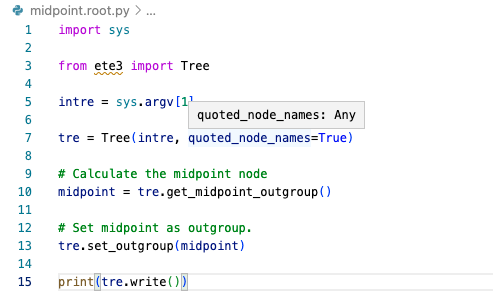
\includegraphics{img/midpoint.root.image.png}
\caption{Python script to midpoint root a tree}
\end{figure}

    Run this script to midpoint root the tree.

    \begin{tcolorbox}[breakable, size=fbox, boxrule=1pt, pad at break*=1mm,colback=cellbackground, colframe=cellborder]
\prompt{In}{incolor}{ }{\boxspacing}
\begin{Verbatim}[commandchars=\\\{\}]
python\PY{+w}{ }midpoint.root.py\PY{+w}{ }gubbins.final\PYZus{}tree.tre\PY{+w}{ }\PYZgt{}\PY{+w}{ }gubbins.final\PYZus{}tree.midpoint.tre
\end{Verbatim}
\end{tcolorbox}

    Visualise this in figtree.

Another common strategy for rooting the tree is \textit{outgroup rooting}.
This is the preferred approach for bacterial datasets. Outgroup rooting
involves including one or more sequences in the analysis that are more
distantly related to our sequences of interest than they are to one
another. These sequence are usually referred to as \textit{outgroups}. The
root estimate is then simply the point at which the outgroup(s) join the
tree. The best possible outgroups are those available which are most
closely related to our sequences of interest but still different enough.
For examples, in this dataset we could use a \textit{Salmonella paratyhi A
sample} as an outgroup.

    There are a few ways to do this. One is to obtain sequence data for the
outgroup sample and incorporate it into the dataset from the beginning
of the analysis and construct a pseudogenome for the outgroup. If no
sequence data is available, you can take a complete reference genome for
the outgroup and \texttt{shred} it to simulate sequencing reads for the
reference. Just remember when calculating and reporting the number of
variant sites for your dataset that you remove the outgroup from the
alignment.

    \hypertarget{clean-up}{%
\subsubsection{Clean-up!}\label{clean-up}}

Clean up any intermediate files that were generated during the analysis
that you no longer require. This is always an important last step of any
analysis as sequence data analysis files can use up large amounts of
disk space. Let's look at what files were created in our analysis

    \begin{tcolorbox}[breakable, size=fbox, boxrule=1pt, pad at break*=1mm,colback=cellbackground, colframe=cellborder]
\prompt{In}{incolor}{ }{\boxspacing}
\begin{Verbatim}[commandchars=\\\{\}]
\PY{n+nb}{cd}\PY{+w}{ }..
ls\PY{+w}{ }\PYZhy{}alhrt\PY{+w}{ }*/*
\end{Verbatim}
\end{tcolorbox}

    As you can see the data analysis has generated a lot of files! So let's
remove any files that do not need to be kept long term:

    \begin{tcolorbox}[breakable, size=fbox, boxrule=1pt, pad at break*=1mm,colback=cellbackground, colframe=cellborder]
\prompt{In}{incolor}{ }{\boxspacing}
\begin{Verbatim}[commandchars=\\\{\}]
rm\PY{+w}{ }fastq/*.trim.fastq.gz
rm\PY{+w}{ }fastq/*.fastp.html
rm\PY{+w}{ }fastq/*.fastp.json
rm\PY{+w}{ }samtools/*.sam
rm\PY{+w}{ }samtool/ERR5243693.bam*
rm\PY{+w}{ }samtools/ERR5243695.bam*
rm\PY{+w}{ }samtools/ERR5243699.bam*
rm\PY{+w}{ }variants/ERR5243693.vcf.gz*
rm\PY{+w}{ }variant/ERR5243695.vcf.gz*
rm\PY{+w}{ }variants/ERR5243699.vcf.gz*
\end{Verbatim}
\end{tcolorbox}

    Now go to the next section: \href{metadata.ipynb}{Phylogeny and
Metadata}


    % Add a bibliography block to the postdoc



\newpage





    \hypertarget{phylogeny-and-metadata}{%
\section{Phylogeny and Metadata}\label{phylogeny-and-metadata}}

Often it is useful to visualise metadata about your samples in the
context of your phylogenetic tree. For example, location information can
provide insight into the processes that drive their epidemiology. This
can be used to infer whether single introductions of a pathogen have
occurred followed by local evolution or whether it transmits frequently
across borders. It can also indicate regions affected by antimicrobial
resistance (AMR).

In this section, you will use \texttt{Microreact} to visualise the
phylogeny you created in the previous section with some basic metadata.
\texttt{Microreact} is software developed by the Centre for Genomic
Pathogen Surveillance (CGPS) that allows you to upload, visualise and
explore any combination of clustering (trees), geographic (map) and
temporal (timeline) data. Other metadata variables are displayed in a
table. You can specify colours and/or shapes to display on the map, tree
and/or timeline. A permanent URL is produced for you to share your
Microreact, or a .microreact file can be downloaded for sharing with
collaborators.

There are several alternatives including FigTree, Phandango and iToL but
for the purposes of this tutorial we will demostrate the use of
Microreact for metadata visualisation.

    \hypertarget{the-dataset}{%
\subsection{The dataset}\label{the-dataset}}

In this section we will make use of a maximum likelihood phylogenetic
tree of the \textit{S. typhi} isolates from the previous section and a
metadata file with information on location, time of isolation and
genotype for the samples.

    \hypertarget{create-a-microreact-project}{%
\subsection{Create a Microreact
project}\label{create-a-microreact-project}}

Start by opening up a new window in Firefox and typing
https://Microreact.org in the address bar. Click on ``Upload'' as shown
below and create a new project.

    \begin{figure}
\centering
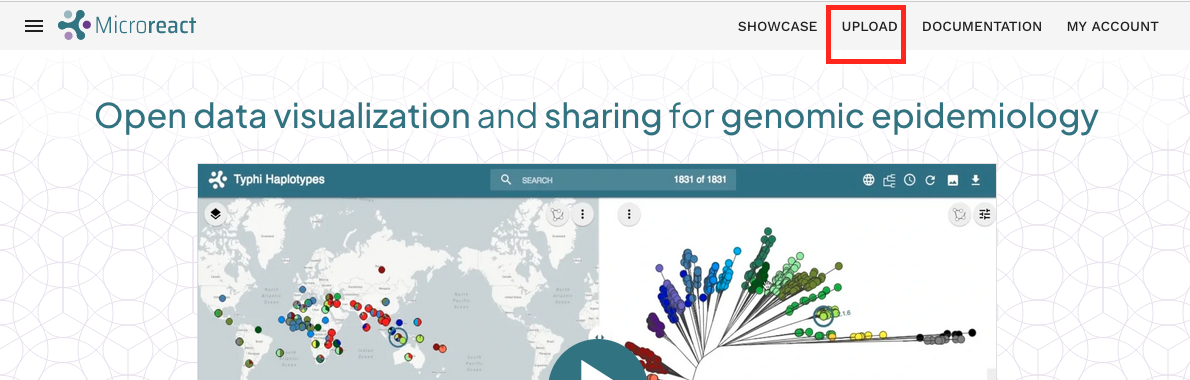
\includegraphics{img/microreact-front-page.png}
\caption{Microreact front page}
\end{figure}

    Open a file browser and navigate to the metadata directory
(\texttt{/home/manager/course\_data/snp\_phylogeny/data/metadata}). Drag
and drop the files ``metadata.csv'' and ``tree.tre'' from the file
browser onto your Internet browser.

    \begin{figure}
\centering
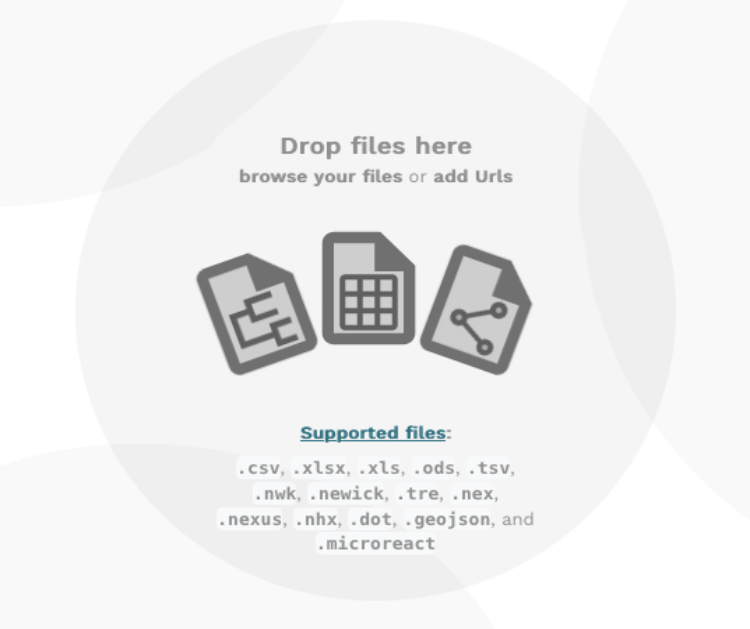
\includegraphics{img/microreact-upload.png}
\caption{Uploading files to Microreact}
\end{figure}

    Once the tree and metadata files are loaded you will be directed to a
new window where files will be automatically detected as Data (CSV or
TSV) file (metadata.csv) and Tree (Newick) file (tree.tre). In this new
window click on `Continue'. In the next window and make sure column `ID'
is selected as the `ID column' and then click on `Continue'.

    \begin{figure}
\centering
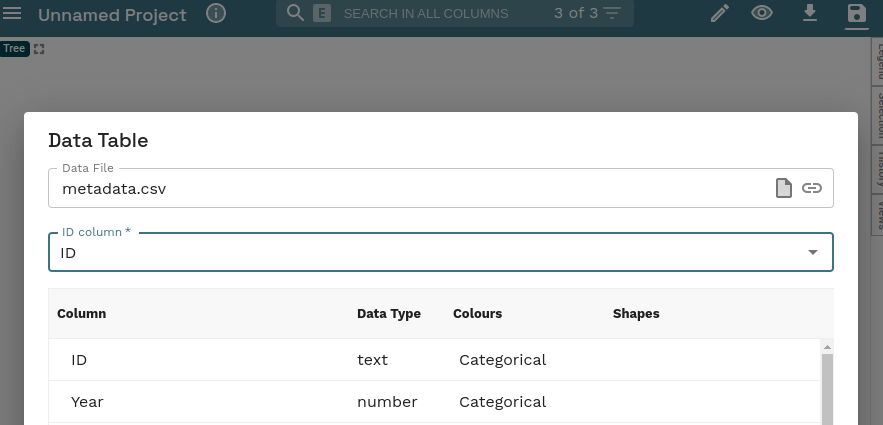
\includegraphics{img/microreact-id.png}
\caption{Selecting sample identifier}
\end{figure}

    Once these forms are completed your data will be utilized to create a
Microreact project. You should now have a view similar to the ones shown
below. You should see a tree view and a timeline and metadata view.

    \begin{figure}
\centering
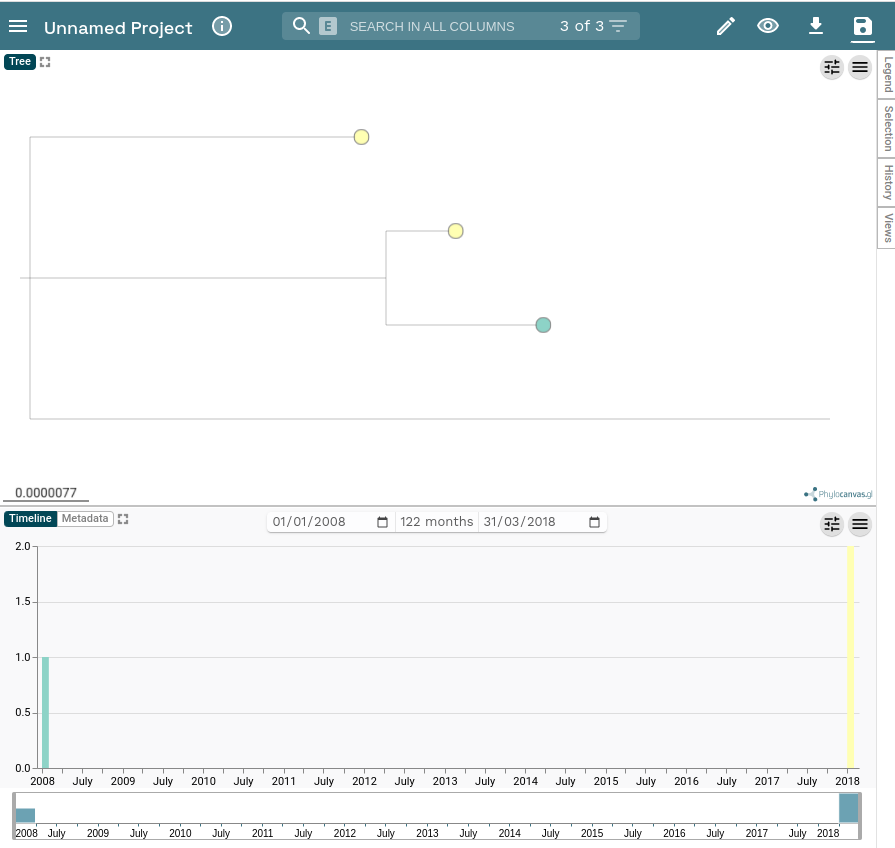
\includegraphics{img/microreact-timeline.png}
\caption{Microreact timeline view}
\end{figure}

    \begin{figure}
\centering
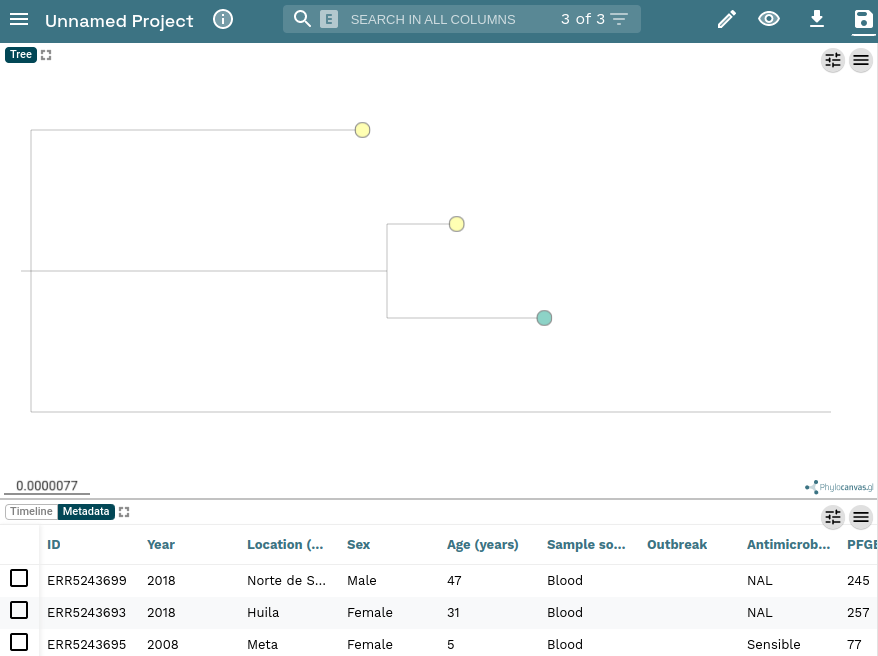
\includegraphics{img/microreact-metadata.png}
\caption{Microreact metadata view}
\end{figure}

    \hypertarget{exploring-the-metadata}{%
\subsection{Exploring the metadata}\label{exploring-the-metadata}}

Clicking on `Show Controls' button in the top right hand corner of the
the tree window allows you to view different kinds of trees and change
text/node size. Try changing layout of the tree.

    \begin{figure}
\centering
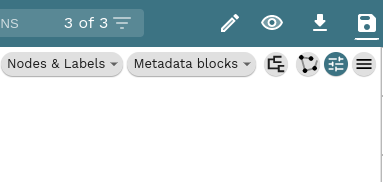
\includegraphics{img/microreact-options.png}
\caption{Uploading files to Microreact}
\end{figure}

    There are lots more things you can do with \texttt{Microreact} but
unfortunately we don't have time to cover them in this tutotial.

\textbf{Congratulations}, you have reached the end of the tutoial!


    % Add a bibliography block to the postdoc



\end{document}
